%----------------------------------------------------------------------------------------
%	PACKAGES AND OTHER DOCUMENT CONFIGURATIONS
%----------------------------------------------------------------------------------------


\documentclass[12pt,oneside,final,a4paper]{report}
\usepackage{generators/imports}
\usepackage{tikz}
\addbibresource{generators/refs.bib}
%\makeglossaries      % alt 1
\makenoidxglossaries  % alt 2

\renewcommand*{\acronymname}{List of Acronyms and Abbreviations}
\renewcommand{\glsnamefont}[1]{\textbf{#1}}

%Create acronyms here.
\newacronym{ide}{IDE}{Integrated Development Environment}
\newacronym{asr}{ASR}{Abstract Semantic Representation}
\newacronym{stf}{STF}{Syntactic Theory Functor}
\newacronym{saas}{SaaS}{Software as a Service}
\newacronym{vcs}{VCS}{Version Control System}
\newacronym{html}{HTML}{HyperText Markup Language}
\newacronym{mvc}{MVC}{Model-View-Controller}
\newacronym{ui}{UI}{User Interface}
\newacronym{dom}{DOM}{Document Object Model}
\newacronym{vdom}{VDOM}{Virtual Document Object Model}
\newacronym{rsms}{RSMS}{Rust Module System}
\newacronym{jsms}{JSMS}{JavaScript Module System}
\newacronym{lsp}{LSP}{Language Server Protocol}
\newacronym{npm}{NPM}{Node Package Manager}
\newacronym{moa}{MoA}{Mathematics of Arrays}
\newacronym{bldl}{BLDL}{Bergen Language Design Laboratory}
\newacronym{vim}{Vim}{Vi Improved}
\newacronym{api}{API}{Application Programming Interface}

%You can also do explanations.
\newglossaryentry{git}
  { name={Git}
  , description={Git is a \gls{vcs} for tracking changes in computer files and coordinating work on those files among multiple people}
  }

\begin{document}
%----------------------------------------------------------------------------------------
%	TITLE PAGE
%----------------------------------------------------------------------------------------

\begin{titlepage} % Create the command for including the title page in the document
  \fontfamily{phv}\selectfont
  \centering % Center all text

  %----------------------------------------------------------------------------------------
  %	TITLE SECTION
  %----------------------------------------------------------------------------------------

  \vspace{200pt}
  {\Huge Developing a zero-core modular IDE} \\ % Title
  \vspace{5pt}

  {\Large \textsl{Creating a zero-cost IDE; you get what you pay for}} % Subtitle or further description
  \vspace{50pt}

  %----------------------------------------------------------------------------------------
  %	AUTHOR SECTION
  %----------------------------------------------------------------------------------------

  \LARGE{\textbf{Nils Michael Fitjar}}\\ % Author name

  \vfill % Whitespace between the author name and the school

  %----------------------------------------------------------------------------------------
  %	DESCRIPTION AND DATE SECTION
  %----------------------------------------------------------------------------------------


  {\Large \textbf{Master's thesis in Software Engineering at} \\
  \vspace{10pt}
  Department of Computer science, Electrical engineering and Mathematical sciences, \\
  Western Norway University of Applied Sciences \\
  \vspace{10pt}
  Department of  Informatics, \\
  University of Bergen \\}
  \vspace{10pt}
  {\large \monthyeardate\today} % Month and year published

  %----------------------------------------------------------------------------------------
  %	LOGO SECTION
  %----------------------------------------------------------------------------------------

  \vfill % Whitespace between the school and the publisher logo


  \begin{figure}[h!]
    \captionsetup[subfigure]{labelformat=empty}
    \subfloat[][]{
\includegraphics[height=70pt]{logos/hvl_logo_engelsk.pdf}}
    \hfill
    \subfloat[][]{
\includegraphics[height=70pt]{logos/uib-logo.eps}}
  \end{figure}


\end{titlepage}

\pagenumbering{roman}

\begin{abstract}
  This paper introduces a modular, \textit{zero-core}, application, to serve as
  an \gls*{ide} for experimental programming languages, addressing limitations
  in traditional \gls*{ide}s. While standard \gls*{ide}s are crucial in software
  development, their support for experimental languages is often inadequate.
  This can be mitigated by extensively using the module
  architecture of existing \gls*{ide}s, by creating specific modules to address
  the shortfall of the host \gls*{ide}. However, relying on \textit{niche}
  modules or functionality is not beneficial for the longevity of the software.
  By analyzing the essential features of traditional \gls*{ide}s a need for
  adaptability by \gls*{ide}s to new paradigms and tools is highlighted. The
  solution, proposed by this paper, is to utilize a modular architecture to
  extend its lifespan and enhance support for experimental languages.
  Magnolia, a research programming language developed at the University of
  Bergen, serves as a case study, highlighting its unique characteristics and
  the necessity for a modular \gls*{ide}. The primary research question explores
  how modularization facilitates the design and implementation of experimental
  programming languages. To showcase the usefulness of a modular approach, the
  modules needed to extend the core application to an \gls*{ide} will be
  implemented.

  \keywords{Modularization \and \gls*{ide} \and Magnolia.}
\end{abstract}

\renewcommand{\abstractname}{Acknowledgements}
\begin{abstract}
  I would like to thank my supervisors, Magne Haveraaen and Mikhail Barash for
  their valuable feedback. I would also like to thank my family, for their
  support throughout my studies. Finally, a thanks to my friends for our long
  lunch breaks.

  \vspace{1cm}
  \hspace*{\fill}\texttt{Nils Michael Fitjar}\\
  \hspace*{\fill}\today
\end{abstract}
\setcounter{page}{1}
\newpage

{
\tableofcontents 
\let\cleardoublepage\clearpage \listoffigures 
\let\cleardoublepage\clearpage \listoftables 
\let\cleardoublepage\clearpage \lstlistoflistings
}
\pagenumbering{arabic}
\setcounter{page}{1}
\setlength{\parskip}{0.5cm plus4mm minus3mm}

\chapter{Introduction}

Standard \gls{ide}s are indispensable tools in modern software development,
offering features like early bug reporting, project outline visualization, code
highlighting, and code completion, however, these \gls{ide}s may not adequately
support the unique demands of experimental programming languages. Experimental
languages could introduce new concepts like \gls{asr} Transformation, Term
Algebras, \gls{moa}, \gls{stf}, or other novel programming features. These are
concepts from the academic community, and are not common in \textit{mainstream}
languages, and as such, have little to no support in modern \gls{ide}s. To solve
this, researchers need ad hoc solutions for existing \gls{ide}s, adding the
needed functionality to test out their language features. If this ad hoc
solution is too extreme; outside the standard functionality supported by the
developers of the \gls{ide}, it might be short-lived. As the \gls{ide} is
maintained, updated and improved, the features used to solve the niche needs of
the experimental language might be deprecated.

However, if the \gls{ide} has integrated support for extending the standard
functionality of the application, then the ad hoc solution will be more stable.
Such a system is known by many names. Plug-in architecture, exstension
\gls{api}, or add-on system, to name a few. The common factor amongst these
systems, is that some component, be it a plug-in, an exstension, an add-on, or a
module, can extend the functionality of the application. This is a modular
approach to extending the lifetime of an application; extending its software
longevity. In many of these systems, said components, are composable,
allowing for multiple components to work together in a modular fashion to add
extra features to an application. This way of adding functionality to an
application is commonly used in \gls{ide}s.


\section{Modular Architecture}

A modular \gls{ide} would assist in these ad hoc solutions. Even if a new
feature from an experimental language is introduced, it is unlikely that this
feature has no relation to existing features, and as such, it is easier to
extend the application in such a manner to facilitate this new feature, with help of
existing modules. However, if it is the case that this feature is
paradigm-shifting, then there will still be existing functionality that can be
used, re-used or extended to facilitate this.

\begin{hyp} \label{hyp:modular}
  When an application is designed to be modular from the start, then features
  not thought of, by the original developers can be integrated into the
  application, and be stable. If an experimental research language introduces
  some paradigm shifting concept, then this can easily be tested in a modular
  \gls{ide}.
\end{hyp}

\section{Zero-core Application}

Taking the modular architecture design to the extreme, the core application has
no base features, everything is enabled by an external module. We call such a
highly modular application, a \textit{zero-core} application. To qualify for a
\textit{zero-core} application, the default application has no functionality;
everything is acquired by modules. Such a design facilitates a modular approach,
enabling a module-developer to only focus on the functionality they want to
extend, not the entire core.

\section{Thesis Outline}

Traditional \gls{ide}s encompass essential features such as syntax highlighting,
code navigation, and hover-help, all of which play a crucial role in the
software development process. However, their limitations become apparent when
working with experimental languages. This paper advocates for modularization and
composability as key design principles, demonstrating their ability to extend
the operational lifespan of software by allowing for ease-of adoption to new
paradigms and tools. The discussion revolves around Magnolia, an experimental
research programming language developed by \gls{bldl} at the University of
Bergen. Magnolia is a way to experiment with novel language features. It will
therefore be a case study illustrating the need for a specialized \gls{ide}. To
achieve this in a sufficient manner, a more specialized \gls{ide} is required.

The focus point of this paper is to design a zero-core architecture, to develop
and implement a modular \gls{ide}, where the target language will be Magnolia.

In chapter \ref{cha:background}, we will introduce Magonlia, and features this
language introduces that are difficult to encompass using standard \gls{ide}s.
In chapter \ref{cha:ide} we will explore the use case of the afformentioned
\gls{ide}, focusing on the different users of such an application. Chapter
\ref{cha:impl} the design and implementation of the \gls{ide}, mentioning
different designs that were considered, and some challanages that were
encountered.


\chapter{Background} \label{cha:background}

\section{Magnolia}

Magnolia is an experimental research language being developed \gls{bldl} at the
University of Bergen. Magnolia is designed to support a high level of
abstraction and ease of reasoning. This is achieved by \textit{concepts},
\textit{axioms}, \textit{satisfaction}, and \textit{implementations}.

\subsection{Magnolia Concept}

Something, Something, \dots, concepts declare types, functions and properties
which those functions need to uphold. A simple example of this would be a
concept for addition with natural numbers.

\begin{center}
  \lstinputlisting
    [ language=Magnolia
    , caption={Natural numbers (Magnolia)}
    , label=lst:nat
    ]{./code/magnolia-nat.mg}
\end{center}

In the listing \ref{lst:nat}, we are specifying concept called
\textit{NaturalNumbers}, which declares a type \textbf{N}, and three methods
that act upon the type \textbf{N}. We have the function, (also called a
constructor), \textbf{zero}, which takes zero arguments, and should return
something of type \textbf{N}. With this constructor, we can instantiate our
numbers. To get new numbers, we have the function \textbf{succ}, which should
give the \textit{succ}essor to the passed number. That way, we can represent $0$
as \textbf{zero()}, $1$ as \textbf{succ(zero())}, and $2$ as
\textbf{succ(succ(zero()))}. The final function, is an infix operator. $+$ takes
two arguments, of type \textbf{N}, and returns an \textbf{N}. Of course, this
should be interpreted as addution, meaning \textbf{succ(zero())} $+$
\textbf{succ(succ(zero()))} $=$ \textbf{succ(succ(succ(zero())))}, or using
numbers: $1 + 2 = 3$. Finally, the last statement in the concept, is an axiom,
stating that given any $a$, if we add \textbf{zero()} to $a$, we should get $a$.
However, this interpretation depends on our implementation
of the concept.
\todo{Add more examples showcasing what is needed from a Magnolia IDE}
\todo{Renaming}
\todo{Showing all imports are DAG's}

\subsection{Magnolia Implementation}

As one can see in listing \ref{lst:impl}, we have implemented the concept
specified in \ref{lst:nat}, by using concrete values for \textbf{N}. There is an
implementation for all the functions, giving us the functionality we set out to
specify with our concept, but there is nothing stopping us from straying away
from the specification, by implementing it incorrectly. As can be seen in
listing \ref{lst:impl-wrong}.
\todo{Add more examples showcasing what is needed from a Magnolia IDE}

\begin{center}
  \lstinputlisting
    [ language=Magnolia
    , caption={Natural numbers implementation (Magnolia)}
    , label=lst:impl
    ]{./code/magnolia-add.mg}
\end{center}

\begin{center}
  \lstinputlisting
    [ language=Magnolia
    , caption={Invalid implementation (Magnolia)}
    , label=lst:impl-wrong
    ]{./code/magnolia-add-wrong.mg}
\end{center}

Here we have implemented our addiction operator in such a way, where it breaks
our axiom. This is where the \textit{satisfaction} comes in, it is what ties the
concept and implementation together, by ensuring our axiom are upheld.


\subsection{Magnolia Satisfaction}

\begin{center}
  \lstinputlisting
    [ language=Magnolia
    , caption={Satisfaction of the natural numbers (Magnolia)}
    , label=lst:sat
    ]{./code/magnolia-add.mg}
\end{center}

Something, Something, \dots, implementations of concepts need to uphold the
axioms declared in the concept being implemented. This is done by using an
external SMT-solver. Satisfaction, babay
\todo{Cite Beate maybe?}

\todo{
  Expand, maybe exploring generic concepts, axioms and implementation, noting
  how a developer would use Magnolia?
}

\subsection{Mathematics and Programming}

Mathematics is everywhere, and useful. It's not always easy to notice this, but
one thing that helps, is knowing the names of the concepts one encounter. One
can easily understand that knowing simple operations like addition,
multiplication, etc. is useful but for more abstract mathematics, this is
harder. An example of this is abstract algebra, which is the study of algebraic
structures, which are structures that are very common in programming. A
programmer will use these structures more often than not, knowingly or
unknowingly, and a good programmer will explicitly seek these structures out.

An important aspect of development, is logging. Knowing what actions have taken
place is an essential tool when hunting down bugs. A common way to structure
logs, would be composing logs, depending on when they occurred. As a concrete
example, let's say we are making a text editor, and are in the need of a logging
manager, which, among other things, should compose different log statements.
Assuming we have some type \textbf{Log(A)}, where there the type \textbf{A}, is the
result of the computation a given function, we want to be able to compose
different, related, computations. But, importantly, the order of composition
of the \textbf{Log(A)}-type matters. Representing the composition of the
\textbf{Log(A)}-type as $\odot$, doing, and letting $a, b, c$ be of type
\textbf{Log A}:

\begin{equation}
  a \odot \left ( b \odot c \right ) = \left ( a \odot b \right ) \odot c
\end{equation}

Now we have a good logger, as the logs of the entire call stack is available for
us to read when something goes wrong. Moving on, a good feature of a text
editor, is being able to undo and redo actions. These are the actions that a
user can do:

\begin{itemize}
  \item Insert text at a position
  \item Delete text from a position
  \item Redo an action
  \item Undo an action
\end{itemize}

Same as in the logging example, composing is a reasonable thing to implement,
and should result in another action. Similarly, the order matters; deleting text
and then inserting, is not the same as inserting and then deleting. But what is
different, is that we also want the \textit{inverse} of an action, so for every
action we want an opposite action that undos an action. Then our composition of
actions looks different. Say, $a$ is some action, and $c$ is some opposite
action, then our composition looks like this:

\begin{equation}
  a \odot c = U
\end{equation}

Where $U$ is an action representing \textit{no-operation}. This could be
inserting the empty string at any position, deleting the empty string at any
position, or redoing or undoing any of the aforementioned actions.

Both of these examples are relatively easy to implement, but harder to verify,
or satisfy our properties; that the \textit{logic} holds. The following are
examples of the logging and editor examples in Java, Rust, and Magnolia
respectively.
\todo{rewrite}

\subsection{Logging example in Java, Rust, and Magnolia}

\todo{Expand}

\begin{center}
  \lstinputlisting
    [ language=Java
    , caption={Logging structure (Java)}
    , label=lst:jlogging]{./code/logging.java}
\end{center}

\begin{center}
  \lstinputlisting
    [ language=Rust
    , caption={Logging structure (Rust)}
    , label=lst:rlogging]{./code/logging.rs}
\end{center}

\begin{center}
  \lstinputlisting
    [ language=Magnolia
    , caption={Logging structure (Magnolia)}
    , label=lst:mlogging]{./code/logging.mg}
\end{center}

\subsection{Editor example in Java, Rust, and Magnolia}

\todo{Expand}

\begin{center}
  \lstinputlisting
    [ language=Java
    , caption={Editor structure (Java)}
    , label=lst:jeditor]{./code/editor.java}
\end{center}

\begin{center}
  \lstinputlisting
    [ language=Rust
    , caption={Editor structure (Rust)}
    , label=lst:reditor]{./code/editor.rs}
\end{center}

In Magnolia, however, this can be enforced on the \textit{interface}-level.
\todo{Rewrite}

\begin{center}
  \lstinputlisting
    [ language=Magnolia
    , caption={Editor structure (Magnolia)}
    , label=lst:meditor]{./code/editor.mg}
\end{center}

The interesting thing about these two structures, is that they are similar,
even though they are used for two different things. Both the logging example,
and the text editor example, are some binary operation over some set. In the
first example, our set was all different log statements of the type
\textbf{Log A}, and composing these logs, gave us another \textbf{Log A} type.
While in the second example, we were working on the set of actions, which we
could compose, which also gave us another action, but we also had an action
representing no-operation, and an \textit{inverse} operation, undoing an action.
This is related to mathematics, specifically abstract algebra, the study of
algebraic structures.

\subsection{Abstract Algebra}

In the first example, we are working with a \textit{semigroup}, and in the
second example, we are working with a \textit{group}. These are known as
algebraic structures, which is just some set, with a binary operation, and some
property on that binary operation. The trivial example, is known as
\textit{magma}, and is defined by \ref{def:magma}. The closure \ref{def:closed}
simply specifies that we only work with one set.

\begin{definition}[Closure] \label{def:closed}
  For a set $M$, with a binary operation $\oplus$,
  $\forall a, \forall b, \exists c \in M$, such that
  $a \oplus b = c$.
\end{definition}

\paragraph{Closure} Addition with the integers, ($\mathbb{Z}$), is a kind of
  closure, as per the definition \ref{def:closed}, since no matter what integer
  you put into the equation, you will still get a positive integer. And since
  this is the only requirement a magma has, this example is also a magma.

\begin{definition}[Magma] \label{def:magma}
  A magma is a set $M$, with a binary operation $\oplus$, which is
  \textit{closed} by definition \ref{def:closed}
\end{definition}

We can \textit{extend} the definition of magma, by adding associativity on the
binary operation. The definition \ref{def:assoc}, as shown in the examples,
simply specifies that the order we evaluate our composition matters.

\begin{definition}[Associativity Law] \label{def:assoc}
  For any binary operation $\oplus$, on a set $M$, $a, b, c \in M$.
  $a \oplus \left ( b \oplus c \right ) = \left ( a \oplus b \right ) \oplus c$,
  must hold.
\end{definition}

This associativity gives us a semigroup, as shown in the definition
\ref{def:semi}, which is the structure that we modeled in our logging example.

\begin{definition}[Semigroup] \label{def:semi}
  A semigroup is a set $M$, with a binary operation $\oplus$, and $\oplus$ must
  uphold the definitions \ref{def:closed} and \ref{def:assoc}.
\end{definition}

\paragraph{Semigroup} Multiplication with the positive integers, ($\mathbb{N}$), is
  associative, since no matter where we put parentheses; what order we
  evaluate this equation: $2 * 3 * 4$, we will get the same answer.

By simply requiring the identity law (\ref{def:ident}), we get a
monoid (\ref{def:monoid}), and adding the inverse law
(\ref{def:inv}), we get a group.

\begin{definition}[Identity Law] \label{def:ident}
  For any binary operation $\oplus$, on a set $M$,
  $\forall a, \exists U \in M$, such that
  $a \oplus U = a$, and $U$ is unique.
\end{definition}

\begin{definition}[Monoid] \label{def:monoid}
  A monoid is a set $M$, with a binary operation $\oplus$, and $\oplus$ must
  uphold the definitions \ref{def:closed}, \ref{def:assoc}, and \ref{def:ident}.
\end{definition}

\paragraph{Monoid} To make a monoid, we can choose the binary operation to be
  $\times$, and our set to be the natural numbers, ($\mathbb{N}$). We know addition
  is closed, and associative, so choosing $U = 1$, we get a monoid. Any number
  from our set $\mathbb{N}$ multiplied with $1$, gives us the number we choose.

\begin{definition}[Inverse Law] \label{def:inv}
  For any binary operation $\oplus$, on a set $M$,
  $\forall a, \exists U \in M$, such that
  $a \oplus U = a$, and $U$ is unique.
  And $\forall a, \exists b \in M$, such that $a \oplus b = U$, and the mapping
  for $a \to b$ is one-to-one.
\end{definition}

\begin{definition}[Group] \label{def:group}
  A group is a set $M$, with a binary operation $\oplus$, and $\oplus$ must
  uphold the definitions \ref{def:closed}, \ref{def:assoc}, \ref{def:ident},
  and \ref{def:inv}.
\end{definition}

The definition \ref{def:group}, of course is identical to the structure we used
to model undo-redo, in our text editor example. To avoid common mistakes when
implementing these structures, it would behoove a developer if they could encode
these properties in something like an interface or a trait, however, this is not
possible in either Java nor Rust.
\todo{Rewrite this}

\todo{Rewrite this to better fit the previous section}

\subsection{Java: Magma to Group}

This structure not could be implemented in something like Java, an
Object-Oriented Language, as shown in listings \ref{lst:jmagma},
\ref{lst:jsemigroup}, \ref{lst:jmonoid}, and \ref{lst:jgroup}. Note the empty
interfaces; there is nothing that enforces the different laws on the properties.
This can only be done by unit testing, which is not enforced on a consumer of
the \gls{api}.

\begin{center}
  \lstinputlisting
    [ language=Java
    , caption={Magma concept (Java)}
    , label=lst:jmagma]{./code/magma.java}
\end{center}

\begin{center}
  \lstinputlisting
    [ language=Java
    , caption={Semigroup concept (Java)}
    , label=lst:jsemigroup]{./code/semigroup.java}
\end{center}

\begin{center}
  \lstinputlisting
    [ language=Java
    , caption={Monoid concept (Java)}
    , label=lst:jmonoid]{./code/monoid.java}
\end{center}

\begin{center}
  \lstinputlisting
    [ language=Java
    , caption={Group concept (Java)}
    , label=lst:jgroup]{./code/group.java}
\end{center}

\subsection{Rust: Magma to Group}

\todo{Expand}

\begin{center}
  \lstinputlisting
    [ language=Rust
    , caption={Magma (Rust)}
    , label=lst:rmagma]{./code/magma.rs}
\end{center}

\begin{center}
  \lstinputlisting
    [ language=Rust
    , caption={Semigroup (Rust)}
    , label=lst:rsemigroup]{./code/semigroup.rs}
\end{center}

\begin{center}
  \lstinputlisting
    [ language=Rust
    , caption={Monoid (Rust)}
    , label=lst:rmonoid]{./code/monoid.rs}
\end{center}

\begin{center}
  \lstinputlisting
    [ language=Rust
    , caption={Group (Rust)}
    , label=lst:rgroup]{./code/group.rs}
\end{center}

\subsection{Magnolia: Magma to Group}

In Magnolia, however, this can be enforced on the \textit{interface}-level. The
example code shown in listing \ref{lst:magma}, showcases a concept
representation a binary operation, which has one function, \textit{binop}, which
takes in two values of type \textit{T}, and returns \textit{T}. Note that the
actual implementation of this function is missing. This is because a concept
encodes the properties of a users code. The actual implementation of the
binary function needs to uphold the properties of the concept that is
being implemented. Note that this is unlike the Java and Haskell example, in
which we have no way to encode the property of our binary function. So any
consumer of our \gls{api} would not be explicitly bound to our restriction of
the associativity law \ref{def:assoc}, identify law \ref{def:ident}, and the
inverse law \ref{def:inv}, required by semigroup and group. The closure
definition, \ref{def:closed}, however, can be encoded by the type system in Java
and Haskell.

\begin{center}
  \lstinputlisting
    [ language=Magnolia
    , caption={Magma (Magnolia)}
    , label=lst:magma]{./code/magma.mg}
\end{center}

In the example code shown in listing \ref{lst:semigroup}, the \textit{magma}
concept has been expanded upon, still following the same rules as before, but
with the added property of associativity.

\begin{center}
  \lstinputlisting
    [ language=Magnolia
    , caption={Semigroup (Magnolia)}
    , label=lst:semigroup]{./code/semigroup.mg}
\end{center}

\begin{center}
  \lstinputlisting
    [ language=Magnolia
    , caption={Monoid (Magnolia)}
    , label=lst:monoid]{./code/monoid.mg}
\end{center}

\begin{center}
  \lstinputlisting
    [ language=Magnolia
    , caption={Group (Magnolia)}
    , label=lst:group]{./code/group.mg}
\end{center}

So Magnolia facilitates reuse, and extension of logic. \todo{expand}

\section{Reusable Software}

One of the most important features in any programming language, is the notion
of \textit{reusability}. From the invention of the GO-TO-statement,
to functions, and external libraries, being able to reuse existing software is
an important tool for a developer. It avoids \textit{re-inventing the wheel}, as
common functionality can be externalized and reused in several different places.
\todo{Can probably expand this by going more in depth}

\subsection{Reuse in Magnolia}

Reusability is also an important feature in Magnolia, but this reusability is in
the entire language. In libraries in other languages, functions are reused, in
an attempt to avoid common logical mistakes, but these mistakes could still be
there, hiding in plain view. In Magnolia, one can re-use the \textit{logic} of a
\todo{Expand}
function. The logging and group example can be rewritten using Magnolia concepts
as shown in listing \ref{lst:logging} and \ref{lst:editor} respectively, by
reusing the concepts we created for semigroup in listing \ref{lst:semigroup} and group
in listing \ref{lst:group}.

\begin{center}
  \lstinputlisting
    [ language=Magnolia
    , caption={Logging example (Magnolia)}
    , label=lst:logging]{./code/logging.mg}
\end{center}

\begin{center}
  \lstinputlisting
    [ language=Magnolia
    , caption={Editor example (Magnolia)}
    , label=lst:editor]{./code/editor.mg}
\end{center}

Here we have used the \textit{renaming} of concepts in Magnolia, where we can
rename types and functions to be more specific, for the specialized use case the
concept is reused in.

\subsection{Software Longevity}

Most examples of \textit{popular} software, are open source, like \gls{vim}.
\gls{vim} is a text editor which has been in use since 1991. There are several
factors behind this success, but the ones being highlighted here, are due to its
extensibility and due to it being open-sourced. Being open sourced, allows for a
rotating cast of maintainers, ensuring the core application has the features its
users wants. The users of \gls{vim} can be split into two categories,
\textit{standard users}, and \textit{module developers}. \gls{vim} has an
extensive module ecosystem, which can extend \gls{vim}s functionality from a
text editor, to a fully fledged \gls{ide}.
\todo{Currently, a weak argument for modularity}
\todo{Mention Eclipse and IntelliJ here as well?}

\section{Integrated Development Environment} \label{sec:ide}
\todo{Turn each paragraph into a subsection?}

An \gls{ide}, aids a developer, as all the needed tools for development are
\todo{Mention the tools, and how devs had it before.}
integrated into one application. There are two different kinds of \gls{ide}s,
generic and specialized. \todo{Source}

A specialized \gls{ide} is one targeted towards a specific language, like
Eclipse, (reference?), or IntelliJ (reference?), which target Java/JVM. It
contains specialized features like the following:
\todo{
  Rewrite this because Eclipse, while generic, has plugin support which, allows
  it to support different languages, as does IntelliJ.
}

\paragraph{Syntax Highlighting} Highlighting important keywords, identifiers
and more, makes the language easier to read for the developer, allowing them to
spot easy to miss errors, like misspelling of keywords, functions, and
variables.

\paragraph{Code Autocompletion} Suggesting keywords, method names or even entire
code snippets, is a powerful tool an \gls{ide} can have. This is possible to
achieve, in some form, without being specialized, by for example, suggesting
text that already exist in the document, but is most useful if it is
specialized, and can suggest built-in methods. This allows a developer to not
having to remember exactly how methods are named, is the method to split a
string by some delimiter, \textit{split\_by} or \textit{split\_on}? As long as
the developer writes \textit{split}, the correct method name will be suggested.

\paragraph{Go-To-Definitions} Being able to quickly navigate to methods and read
their implementation is a useful tool for a developer, as less time has to be
spent navigating the project structure, to figure out where some method was
implemented, and more time can be spent actually developing.

\paragraph{Pretty Printing/Formatting} Following the languages style guide.
\todo{Expand, add examples like with Rust}

\paragraph{Boilerplate Code Generation} For unit tests, getters and setters,
(where relevant), and similar.

A lot of these features are possible due to \gls{lsp} which allow for a
standardized way for compilers to give code-support to \gls{ide}'s.

A generic \gls{ide} contains the features that are common among development in
any programming language, like:

\paragraph{File Explorer} Most project nowadays is larger than one file, so
being able to visualize the project in a tree-like-structure, and navigate that,
is useful. This feature usually comes with the ability to manipulate the project
structure, by adding files, folders, moving files around, and deleting them.

But creating any \gls{ide} would still limit the lifetime of the \gls{ide}.
The best example of a long living active \gls{ide}, or, at least editor, is Vim
(source?). Vim is not a feature full editor, but it is simple, lightweight, and
works on any operating system. But most people use it, for how easy it is to
extend; Its lifetime has been greatly extended by the ease of modularization.
Any popular module for Vim is open-source, and therefore, if any module had an
active community around it, if the \textit{lead} developer of the module stopped
developing it, that community can continue to develop the module, either by
getting maintenance access to the repository, or by forking it. Ensuring the
lifetime of the module is extended.

\section{Module Architecture}

\todo{Talk about modules in IDEs}

A modular application, is an application which can be extended by other pieces
of software. This extensibility is useful as features that the original
developers of the application did not think about, can be added. If this module
architecture is well-designed, then this extension can be added without changing
the core application.

There are different ways an application can be extended. The most common one
uses so-called \textit{live-reload}, in which, if a module drastic changes the
functionality of an application, the application has to be restarted, or if it
is a \textit{minor} change, the module is simply loaded. This method is
extending the application during runtime, which is the method most users
expect. Another method would be \textit{compile-time-extension}, in which
modules are added before the application itself is compiled. There are some
advantages and disadvantage in all approaches.

Something, something \dots, in Eclipse modules extending modules is quite
common, using Eclipse Rich Client Platform. \cite{eclipseRcp}

\subsection{Compile Time Module}

\todo{Expand}
As an example, a standard user of any application will expect the application to
come bundled with all the needed functionality. This is best achieved with the
\textit{compile-time-extension} method, since the application can be installed
with the expected modules. A compile time module is usually made using the same
language as the core application.
\todo{Maybe mention it could be faster due to compiler optimalization?}

\subsection{Runtime Module}

\todo{Expand}

Runtime modules are usually also interpreted, but they can still be a
library, same as in a compile time module.

\subsection{Module Ecosystem}

\todo{Expand}
More modules == better, right?

In modern \gls{ide}s, with an extensive module architecture, there exists a
vast module ecosystem. From simple modules that change the color scheme, or
add file icons to more complex modules that add support for other languages.
A good variety of a module ecosystem can help ensure the longevity of an
\gls{ide}. In the table \ref{tbl:mod}, we can see that \gls{ide}s have an
extensive module architecture. \footnotemark

\footnotetext{
  \unskip Data found by looking at the marketplace\footnotemark for the modules,
  \unskip in order:
  \unskip \url{https://marketplace.eclipse.org/content/welcome-eclipse-marketplace}% Eclipse
  \unskip, \url{https://plugins.jetbrains.com/} % Intellij
  \unskip, \url{https://github.com/search?q=vim+plugin\&type=repositories} % Vim
  \unskip, \url{https://github.com/search?q=nvim+plugin\&type=repositories} % Nvim
  \unskip, \url{https://marketplace.visualstudio.com/search?target=VSCode\&category=All\%20categories\&sortBy=Installs} % vscode
}

\begin{table}[]
  \centering
  \caption{Module Ecosystem per \gls{ide}}
  \label{tbl:mod}
  \begin{tabular}{|l|l|}
    \hline
    \gls{ide} & Module count \\ \hline
    Eclipse & $\sim1200$ \\ \hline
    Intellij & $\sim9500$ \\ \hline
    \gls{vim} & $\sim11500$ \\ \hline
    Nvim & $\sim16100$ \\ \hline
    VS Code & $\sim71700$ \\ \hline
  \end{tabular}
\end{table}

\footnotetext{
  Nvim and Vim's marketplace is GitHub, so the results are found by searching
  GitHub for Nvim plugins and Vim plugins respectively, furthermore, all Vim
  plugins can be used by Nvim.
}

\subsubsection{Module Marketplace}

It is important to be able to get modules.

\todo{Mention the need for a module marketplace}

\subsection{Granularity}

When designing modules, the \textit{granularity} of the combined modules has to
be considered. As an example, if one where to extend the zero-core application
with the needed functionality for it to be considered an \gls{ide}, this could be
achieved by creating a singular module which does all the work. However, this
is not a modular approach, as if one wants to change some specific feature in
the \gls{ide}-module, one would have to re-create the whole module with that
specific feature implemented. Instead, if this functionality was granular,
that is to say, split into several modules, that together enable the needed
features, then it would be \textit{simpler} to modify the needed modules to
achieve the wanted feature.


\subsection{Module Family}

\todo{
  Redo this to be less specific, then add a specific section, which reflects
  what has been done
}

\begin{figure}
  \centering
  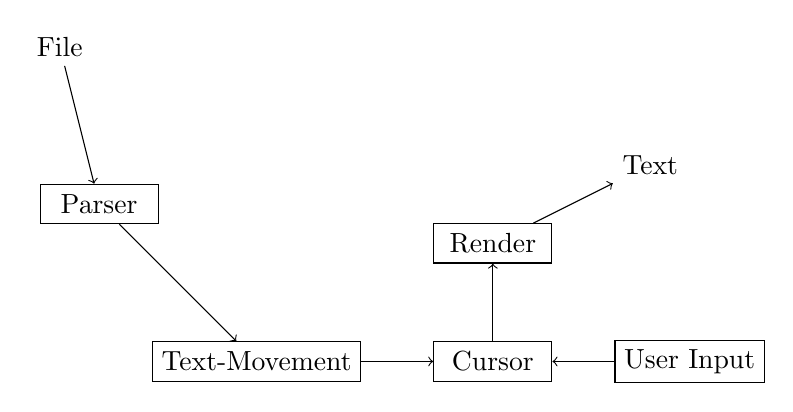
\begin{tikzpicture}
  % Nodes
  \node (file) [] at (-6, 3) {File};
  \node (parser) [rectangle, draw, minimum height=0.5cm, minimum width=1.5cm] at (-5.5, 1) {Parser};
  \node (text-movement) [rectangle, draw, minimum height=0.5cm, minimum width=1.5cm] at (-3.5, -1) {Text-Movement};
  \node (cursor) [rectangle, draw, minimum height=0.5cm, minimum width=1.5cm] at (-0.5, -1) {Cursor};
  \node (user-input) [rectangle, draw, minimum height=0.5cm, minimum width=1.5cm] at (2, -1) {User Input};
  \node (render) [rectangle, draw, minimum height=0.5cm, minimum width=1.5cm] at (-0.5, 0.5) {Render};
  \node (text) at (1.5, 1.5) {Text};
  % Arrow
  \draw[->] (file) -- (parser) node[midway, above] {};
  \draw[->] (parser) -- (text-movement) node[midway, above] {};
  \draw[<-] (cursor) -- (text-movement) node[midway, above] {};
  \draw[<-] (cursor) -- (user-input) node[midway, above] {};
  \draw[->] (cursor) -- (render) node[midway, above] {};
  \draw[->] (render) -- (text) node[midway, above] {};
\end{tikzpicture}

  \caption{Text Editor Module Family}
  \label{fig:textEditorSimple}
\end{figure}

In figure \ref{fig:textEditorSimple}, an input file is parsed to some structure
which is used to translate user actions, into cursor movements. The cursor being
the place in the file where text is written to by the user.

This is a feature that naturally shows up in a \textit{true} modular system. If
several modules together enable some feature, then those modules can be treated
as a singular module by an external module developer, depending on what they
want to extend.


\section{Language Workbench}

Language workbenches are environments for simplifying the creation and use of
computer languages. \cite{lwb}

\todo{Expand}

\section{Language Server}
\todo{Go more in depth about language server stuff}
The most important features in a modern \gls{ide} are possible due to the
\gls{lsp}. \gls{lsp} is a protocol for a language server and editor,
(the client), with which they communicate, allowing for many of the features
mentioned in section \ref{sec:ide}, and explicitly mentioned in table
\ref{tbl:ide}. \gls{lsp} being the standard since the 2020s, is a sign of
modularity being preferred, as now a single \gls{lsp} can be created, and used
across several different applications, like IntelliJ, VS Code and \gls{vim}.
While useful for \textit{standard} language, this is the limiting factor when it
comes to supporting experimental languages, as not only does a new set of
protocols need to be appended to a language server, the editor itself needs to
be changed to actually use these protocols. This creates a lot of work, for both
the \gls{ide} developer and for the compiler developer. Here is where a modular
approach can help both. If some new functionality or feature is added to the
experimental language, this off course means the compiler/interpreter has to be
expanded and/or modified, but for the \gls{ide}, a module could be added and/or
modified to utilize this change, instead of having to change the entire
application.

\begin{table}[]
  \centering
  \caption{\gls{ide} features enabled by \gls{lsp}}
  \label{tbl:ide}
  \begin{tabular}{|l|l|}
    \hline
    IDE Feature & \gls{lsp}-method \\ \hline
    Go to Declaration & textDocument/definition \\ \hline
    Go to Implementation & textDocument/implementation \\ \hline
    Auto-completion & textDocument/completion \\ \hline
    Hover & textDocument/hover \\ \hline
    Warnings & textDocument/publishDiagnostics \\ \hline
    Rename & textDocument/rename \\ \hline
  \end{tabular}
\end{table}

\section{Existing Magnolia IDE}

The current \gls{ide} for Magnolia \cite{baggeIde}, is a many-years-old version
of Eclipse, using modules and functionality from the core Eclipse application,
that has since been outdated. The \gls{ide}s lifetime was limited by a
dependency on external modules and features that where not maintained by the
\gls{ide}-developers. This meant that for future development of Magnolia, an
outdated \gls{ide} was needed, with outdated tooling. Furthermore, the Magnolia
\todo{This could be its own section, maybe?}
compiler was implemented as an Eclipse module, which means that development is
limited to Eclipse, and only Eclipse, as a developer cannot compile Magnolia
code without it.

Modularization will help to mitigate some of the issues with the current
Magnolia \gls{ide}. Instead of maintaining an entire application, the needed and
wanted features of the application can be maintained instead.

Experimental languages might have features which are not possible to be fully
used in current \gls{ide}s. This is also the case for the current Magnolia
\gls{ide}. The compiler for Magnolia, syntax highlighting, error reporting, and
hover-functionality are functionality made in the Eclipse \gls{ide}, by using
its plug-in architecture. Some of the functionality and plug-ins this
implementation used, have been deprecated in later version of Eclipse. This
means the Magnolia \gls{ide} is locked to an old version of Eclipse, which, as
time passes, increases the complexity of installation, as the surrounding
tooling and libraries needed by this version of Eclipse also becomes deprecated.
Currently, in INF220, at the university, two weeks are set aside for students to
be able to install it.

\section{Challenges imposed by Magnolia}

In most programming languages, any type has a singular definition, so invoking
the \textit{go-to-definition} endpoint implemented by an \gls{lsp} results in a
singular response. The actual response of the \gls{lsp} is a list, but this is
\textit{always} a singleton. However, in Magnolia a singular type could have
multiple definitions, and resolving this can be complex.

\subsection{Renaming}

As shown earlier, in Magnolia, one can make some concept, and reuse this concept
in another one. An example of this can be shown in listings \ref{lst:foo}, and
\ref{lst:bar}, where we have the concept \textit{Foo} being used in \ref{lst:bar}.
\todo{Make this true}
\todo{Add a non-empty-list example}

\subsection{Dependency Cycles}

Programming languages have different ways to avoid this problem.
\todo{Figure out what this problem is called}
The easiest, is to simply disallow such import structures, which is something
Magnolia does. All imports have to be \gls{dag}'s. In most programming languages
this is trivial to solve for developers, as if suddenly a project has a cyclic
import, it can be solved quite easily. This could be complex, but in most cases
this is an easy fix. However, due to the heavy reuse in Magnolia, the cycles
could be quite large and harder to reason about without a tool to visualize the
dependency graph.
\todo{rewrite}


Mention \gls{asr}s?

Mention the need for two different external programs, a compiler and a solver?


\chapter{Magnolia IDE} \label{cha:ide}

This chapter will discuss the new Magnolia \gls*{ide}, the different users of the
\gls*{ide}, and their possible experiences which was under consideration when
developing the application.

\section{User Perspectives}

This application has to consider different users. In \gls*{ide}'s like
Eclipse or IntelliJ, there is the primary user base, the developers
who are using the \gls*{ide} to develop, and then there are the secondary user
base, the developers whom develop modules for the \gls*{ide}. Being the
primary user base, most of the new features implemented by either \gls*{ide} are
related to the development experience. There are still changes to that the
module developers are interested in, namely \gls*{api} changes.
IntelliJ for example, lists their \textit{incompatible \gls*{api} changes}\footnote{\url{https://plugins.jetbrains.com/docs/intellij/api-changes-list-2025.html\#intellij-platform-20252}}.
Breaking changes between \gls*{ide} versions is something normal users of the
\gls*{ide} do not worry about. As usually when a new version is released, it
means more features for the developer to utilize. While module
developers have to ensure their modules still work. One of the reasons
behind \gls*{ide} version changes can break a module, is due to how
they interact with their \gls*{ide}. In IntelliJ a module is
created by implementing a Java interface for the functionality one wants.

If one wanted IntelliJ to recognize that a file with the extension "rs",
is a Rust source file, and give it a certain icon, one would have to implement
the \textbf{Language} interface and override the \textbf{getIcon} method to
return the wanted icon.

So a change in the \gls*{ide} architecture could break a \textit{plugin} for the
newer version of the \gls*{ide}, as with Bagge's Magnolia \gls*{ide}~\cite{baggeIde}.
While in this zero-core \gls*{ide} module developers are quite important, as they
are the ones who add the functionality to the \gls*{ide}. Therefore, the core
\gls*{api} has to be more stable, and it is by virtue of not having much
functionality.


\section{IDE Users}

As mentioned in chapter \ref{cha:background}, modern \gls*{ide}s come with an
integrated module architecture. Which is used to extend/change the \gls*{ide},
from as simple as to change the theme, to more drastic changes, like changing
all key binds to \textit{vim-motions}. In any case, a user expects certain
functionality to already exist in an \gls*{ide}, like text editing. A maintainer
of a zero-core \gls*{ide} could supply modules added at compile time, meaning the
expected functionality is there out of the box, while more thematic modules
could be supplied as runtime modules. Example of more functionality based
modules are as follows:

\begin{enumerate}
  \item \textit{ide\_framework}: Responsible for general layout
  \item \textit{ide\_explorer}: Responsible for the file explorer
  \item \textit{ide\_pm}: Responsible for the menu bar
  \item \textit{ide\_tabs}: Responsible for the tabbing system
  \item \textit{ide\_editor}: Responsible for the editor
  \item \textit{ide\_fsa}: Responsible for file system operations
\end{enumerate}

\paragraph{ide\_framework} This module sets up the general \gls*{ui} layout,
which other modules depend on. In the figure \ref{fig:ideLayout}, we have laid
out the naming convention we use when referring to different \textit{places} in
the \gls*{ide}.

\begin{figure}[H]
  \centering
  \begin{tikzpicture}
  \node (window) [rectangle, draw, minimum height=7cm, minimum width=10cm] at (0, 0) {};
  \node (menu) [rectangle, draw, minimum height=0.5cm, minimum width=10cm] at (0, 3.25) {Menu};
  \node (tabs) [rectangle, draw, minimum height=0.25cm, minimum width=8cm] at (1, 2.75) {Tabs};
  \node (tab) [rectangle, draw, minimum height=0.25cm, minimum width=1cm] at (-2.5, 2.75) {Tab};
  \node (sidebar) [rectangle, draw, minimum height=6.5cm, minimum width=2cm] at (-4, -0.25) {Sidebar};
  \node (content) [rectangle, draw, minimum height=6.5cm, minimum width=8cm] at (1, -0.25) {Content};
\end{tikzpicture}
  \caption{
    Diagram of the layout of different areas in our \gls*{ide}
  }
  \label{fig:ideLayout}
\end{figure}

\paragraph{ide\_explorer} In picture \ref{pic:ideEx} we can see the
module, \textit{ide\_explorer} in action, showing the Magnolia library
visualized as a tree-like structure with collapsible folders. These folders are
rendered in the \textit{sidebar}, on the left. When we click on the
\textit{File} button in the menu, a dropdown appears, where we can click on a
button, \textit{Open Folder}, which invokes the ide\_fsa module, the module in
charge of handling file system operations, where we get in \textit{response},
all the folders and files in the path we selected. Which we transform into
\gls*{html}, and along with some \gls*{css}, we get the collapsible folders.

\begin{figure}[H]
  \centering
  
\includegraphics[height=0.5\textwidth]{ide-explorer.png}
  \caption{
    ide\_explorer module, showing the Magnolia library.
  }
  \label{pic:ideEx}
\end{figure}


\paragraph{ide\_pm} Is a module responsible for the menu bar at the top of the
\gls*{ide}. It just simplifies the creation of interactive \gls*{ui} elements
for other modules. The Module has functionality for handling dropdown menus,
which are common in \gls*{ide}-\gls*{ui}s.

\paragraph{ide\_tabs} This module handles pagination of the \gls*{ide}, where
other modules can add their own content to different tabs, that this module can
cycle through. By clicking on a file in the file explorer, a tab is made, where
the contents are managed by the \textit{ide\_editor} module.

\paragraph{ide\_editor} The editor module is coupled with the \gls*{ide}
framework, and the ide\_explorer module. We can open and edit files using the
combination of these modules. By clicking a file in the tree, we can invoke the
ide\_editor module, which invokes the ide\_tabs module, creating a tab with a
text editor in. In picture \ref{pic:editorModule} we can see this in action, as
the editor is created in the \textit{content} place, in the center of the
\gls*{ide}, along with a \textit{tab}, with the name of the file being edited as
the title of the tab.

\begin{figure}[H]
  \centering
  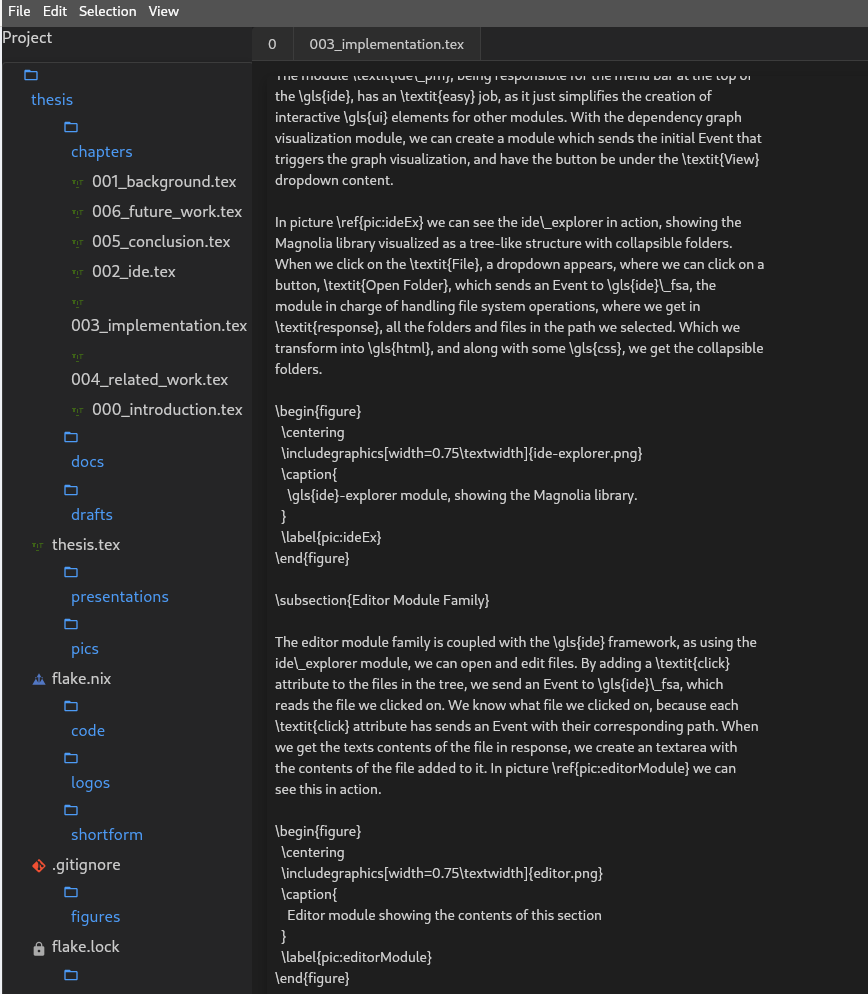
\includegraphics[width=0.5\textwidth]{editor.png}
  \caption{
    Editor module showing the contents of this section
  }
  \label{pic:editorModule}
\end{figure}

\paragraph{ide\_fsa} Since this \gls*{ide} can target different \gls*{os}es, we
need some form of \gls*{fsa}. This is achieved by our module, ide\_fsa, which
enables other modules to do file system operations without having to worry about
what \gls*{os} they are on.


\subsection{Magnolia Dependency Graph Visualizer}

In Magnolia, as in many other languages, one cannot have a cyclic dependency.
This means that the dependency graph of a Magnolia project should be a
\gls*{dag}. And since Magnolia has such a focus on reuse, the dependency graphs
in a Magnolia project could be quite large. Which means the cycles could be
quite long, which would make resolving the cyclic dependency issue complicated.
One way to help a developer, would be to give them a tool to visualize the
dependency graph, so that they could see what modules are connected. Using the
Magnolia library as the input, we can create a visualization of the dependencies
in Magnolia. Using two modules, one for \textit{parsing} the Magnolia library,
finding all packages, and their dependencies, and another for visualizing
this.

The module responsible for rendering the graph, uses
\textit{D3}\footnote{\url{https://d3js.org/}}, a visualization library for
JavaScript. In the picture \ref{pic:magLib}, we can see the finished rendering
of the dependency graph of the Magnolia basic library. As mentioned earlier,
Magnolia has a lot of re-use, and therefore dependencies. That makes this
visualization quite \textit{noisy}, as there are a lot of crossing between the
dependencies.

\begin{figure}[H]
  \centering
  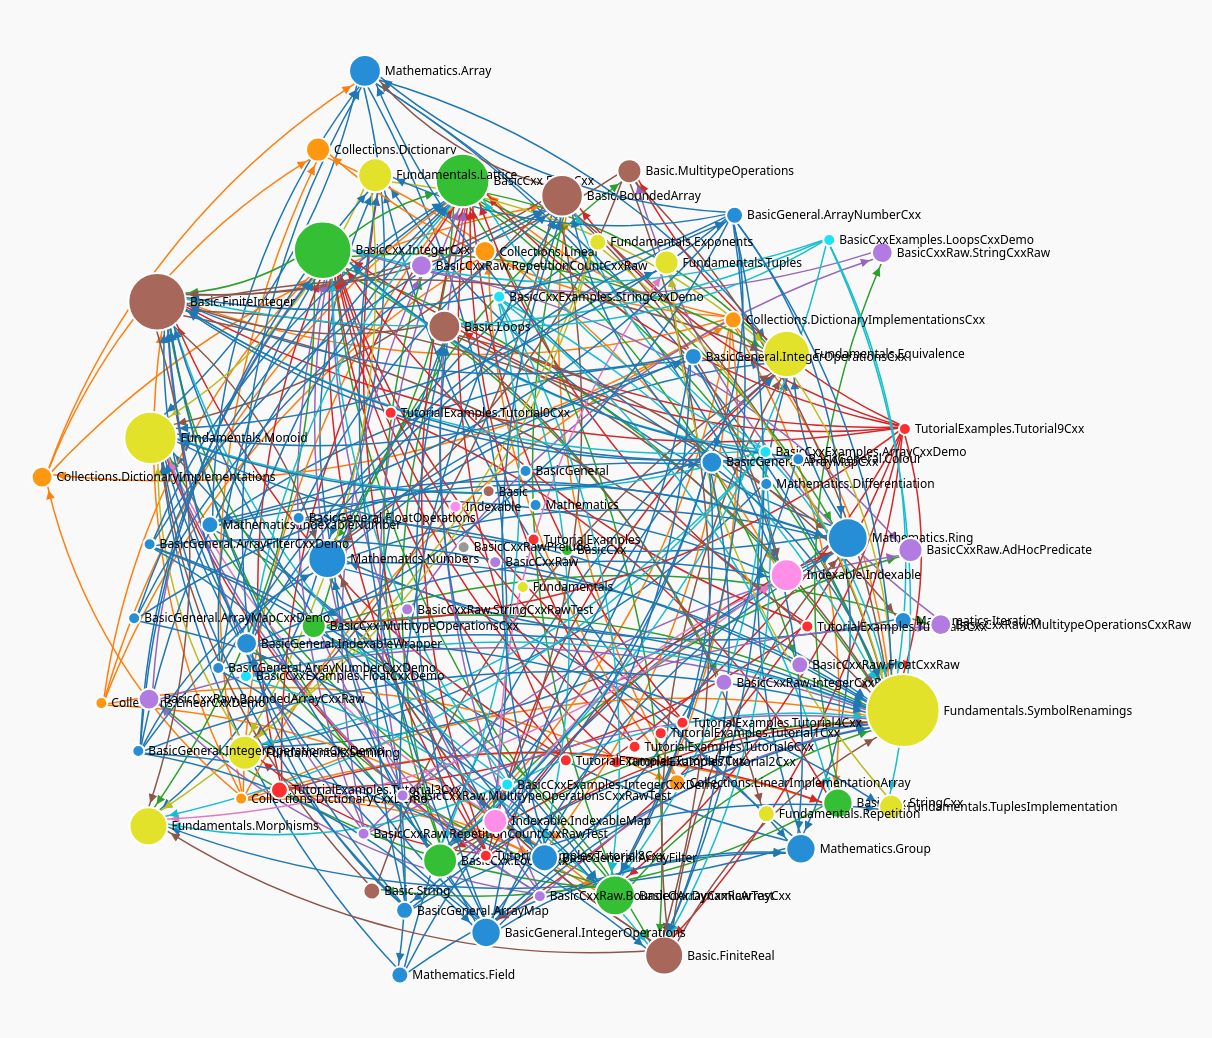
\includegraphics[width=0.75\textwidth]{magnolia-dependencies.png}
  \caption{
    A module that visualizes the dependency graph in the Magnolia basic library.
    Each colour represents a package, which contains several modules. The size
    of the nodes vary depending on the amount of dependents a module has. The
    module utilizes an external JavaScript library to create this visualization.
  }
  \label{pic:magLib}
\end{figure}

Luckily, with D3 and \gls*{css}, we can mitigate some of the noise. In the
picture \ref{pic:depCont}, we can see the control-panel that our graph module
has created. With the control panel, we can zoom in and out on the graph\footnote{This can also be done with the mouse},
and reset our view. This, along with the node size scale, scaling how big
a node is depending on how many dependents it has, ensures this visualization
tool can be used for other programming libraries, not just Magnolia.\footnote{Given a proper parser module}
Furthermore, we can highlight the packages we care about, using the filter
panel the module created. In picture \ref{pic:depFil}, all the different
Magnolia packages have been detected, and their corresponding colour has been
added. We can then enable, or disable them.

\begin{figure}[H]
  \begin{subfigure}[h]{0.45\textwidth}
    \centering
    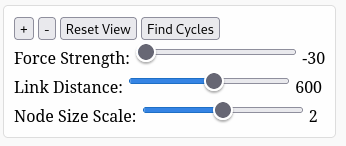
\includegraphics[width=0.85\textwidth]{dependency-viewer-controls.png}
    \caption{
      Control panel, with buttons and sliders for controlling the graph view
    }
  \label{pic:depCont}
  \end{subfigure}
  \hfill
  \begin{subfigure}[h]{0.45\textwidth}
    \centering
    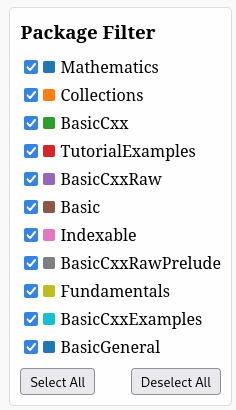
\includegraphics[height=0.8\textwidth]{dependency-viewer-filter.png}
    \caption{List of packages in the graph, that can be toggled}
    \label{pic:depFil}
  \end{subfigure}
  \caption{
    The control panel and package legend, created by the visualizer module.
  }
  \label{fig:foobarbar}
\end{figure}

In the picture \ref{pic:depDis}, we can see the graph after we have disabled all
other packages, except the \textit{Fundamentals} package.

\begin{figure}[H]
  \centering
  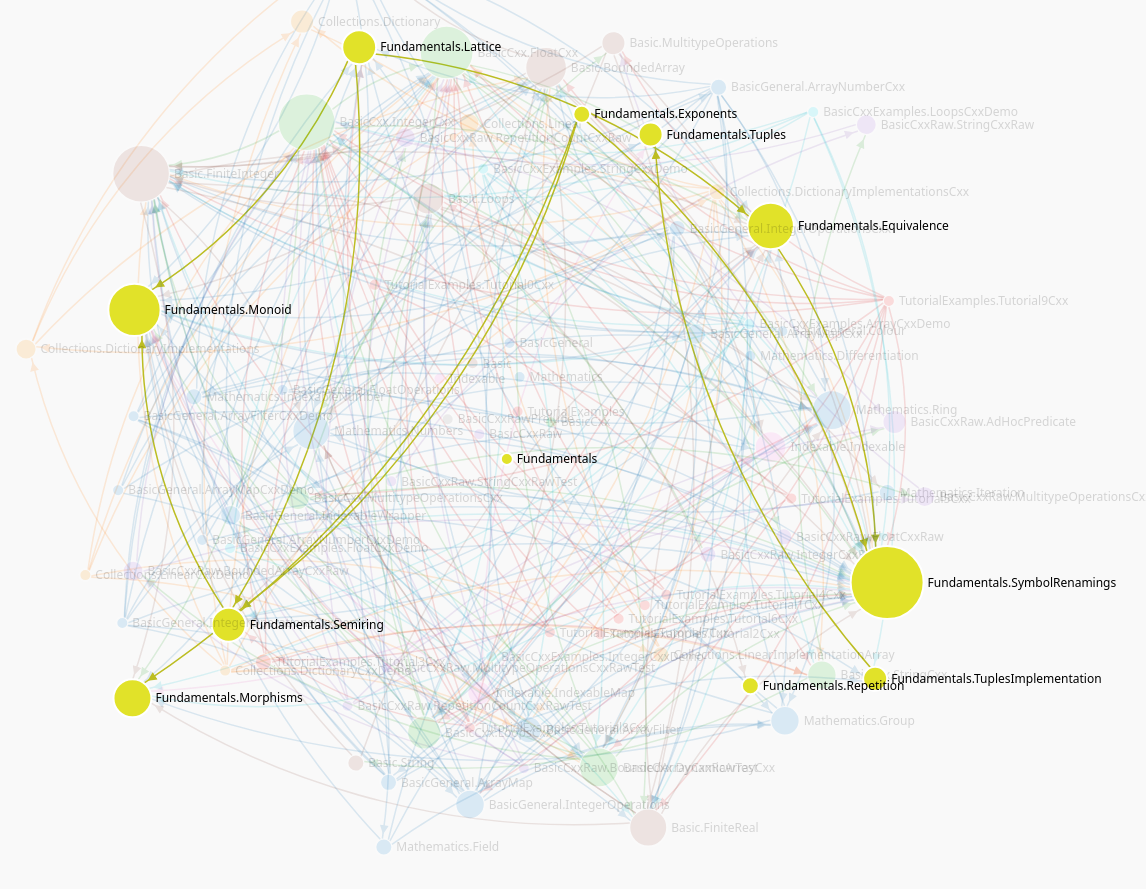
\includegraphics[width=0.75\textwidth]{magnolia-dependencies-filtered.png}
  \caption{
    A module that visualizes the dependency graph in the Magnolia basic library,
    with just the \textit{Fundamentals} package highlighted.
  }
  \label{pic:depDis}
\end{figure}


\subsection{Developer}

Most users just want an \gls*{ide}, and do not spend, nor want to spend, much
time configuring their \gls*{ide}. This can be achieved by adding the necessary
modules to qualify as an \gls*{ide} at compile time. If one is a lecturer,
teaching something that is used by a \textit{niche} programming language, the
lecturer can add the needed modules to a configuration file,
\textit{Modules.toml}, and then compile it to an \gls*{ide}. Before the \gls*{ide}
is compiled, it finds the mentioned modules in the configuration file, and
directly integrates them into the core, ensuring that the resulting binary is a
fully fledged \gls*{ide}. And then this \gls*{ide} can be distributed to the
students, who can still extend the \gls*{ide} with runtime modules at their own
digression.

\subsection{Module Installer}

Module markets are an important part of the \gls*{ide} user experience. Being
able to install a module with the click of a button essential. Not having a
dedicated module market like VS Code, has not been detrimental for
Vim, as with a \textit{plugin manager}, a user can install a module by
simply supplying a URL to a GitHub repository. Similarly, we allow users to
either install modules from disk, or by supplying a URL to a GitHub repository.
In the picture \ref{pic:moduleInstaller}, we can see such a form. A user can
either install a module from disk, in which case, we simply copy the module
binary at the given path to the runtime module folder, or if a URL has been
supplied, we get the latest released binary from that GitHub repository, and
copy this binary instead.

\begin{figure}
  \centering
  
\includegraphics[width=0.50\textwidth]{module-installer.png}
  \caption{
    A module installation form, where a user can supply a path to a module on
    disk, or a URL to a GitHub repository containing the module binary.
  }
  \label{pic:moduleInstaller}
\end{figure}

\section{Module Developer}

Being a zero-core application; all functionality comes from modules, the module
developer experience is the most important. To achieve this, documentation is
important. If a module developer has a question about how the core might react,
it should be answered by the documentation. In Eclipse, this is in the
form of \textit{Javadoc}s, which specify, with examples how the Eclipse
runtime handles \textit{plugins}\footnote{\url{https://help.eclipse.org/latest/rtopic/org.eclipse.platform.doc.isv/reference/api/org/eclipse/core/runtime/Plugin.html}}.

The documentation for \textit{plugin} developers, in both IntelliJ and
Eclipse has to be large, due to of how \textit{plugins} interact with the
\gls*{ide}; it is a large \gls*{api}. In a zero-core \gls*{ide} it is smaller,
simply due to the fact that the core \gls*{ide} offers fewer features, as features
necessarily come from modules in a zero-core architecture.

\subsection{Language Agnostic Modules}

The largest limiting factor in module oriented applications, is the
\textit{language barrier}. Most applications limit what language one can extend
an application with, like in VS Code, where its JavaScript/HTML/CSS. Or
IntelliJ, where one can use Java or Kotlin. But what does language agnostic
mean in the context of our modular architecture? Semantically alike modules.

Translating a module from one programming language to another should be trivial.
This is achieved by the models used in the core. The \textit{primitive} types,
are the same as in JavaScript, the notion of an empty value, numbers, strings,
lists and \textit{objects}, can be serialized/deserialized to/from any language.
So the manipulation on these types can be extracted and rewritten in another
preferred language. Therefore, to be fully language agnostic, modules should be
syntactically translatable between each other. The same two modules, one
implemented in JavaScript, the other in Rust, should be semantically the same.

Of course, this language agnosticism also extends to our libraries. Utility
functions, for manipulation the \gls*{ui} or the primitive types in our state,
should be equivalent, par for naming conventions, as this is a syntactical
difference, not semantically different.


\subsection{Module developer tools}

When developing against a module architecture, having tools to help debug issues
is useful. Common issues when developing in a modular architecture, where
modules can invoke other modules, are incorrect invocation, as in invalid
arguments or return type. Being able to manually invoke modules during runtime
is a great tool for debugging. In picture \ref{pic:eventMock} we can see this a
prototype module where module developers can manually invoke other modules.

\begin{figure}[H]
  \centering
  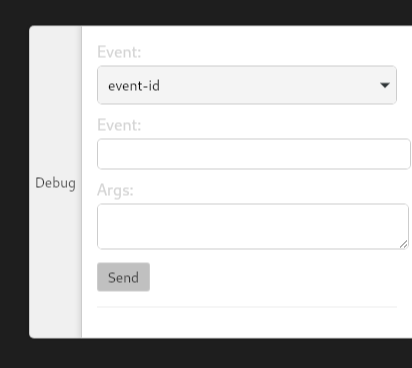
\includegraphics[width=0.5\textwidth]{event-mocking.png}
  \caption{
    Module that adds a simple pop-up menu for manually invoking other modules,
    by using the event system, discussed more in chapter \ref{cha:impl}.
  }
  \label{pic:eventMock}
\end{figure}

When mocking in \gls*{rest}-\gls*{api} development, one creates the expected
response, which is usually a \gls*{json}-file. The same is done here, where the
\textit{Args} field in this form expects the argument to be in \gls*{json}. This
is helpful, as other testing libraries, like \textit{Playwright}, does the same
and the \gls*{ide} logs the arguments in the same formatting, meaning we
can simply copy-paste the argument we want to mock from the logs, into the
field. Another helpful tool, is the one shown in the picture
\ref{pic:debugState}. Here we can see a module which visualizes the current
state of the \gls*{ide}.

\begin{figure}[H]
  \centering
  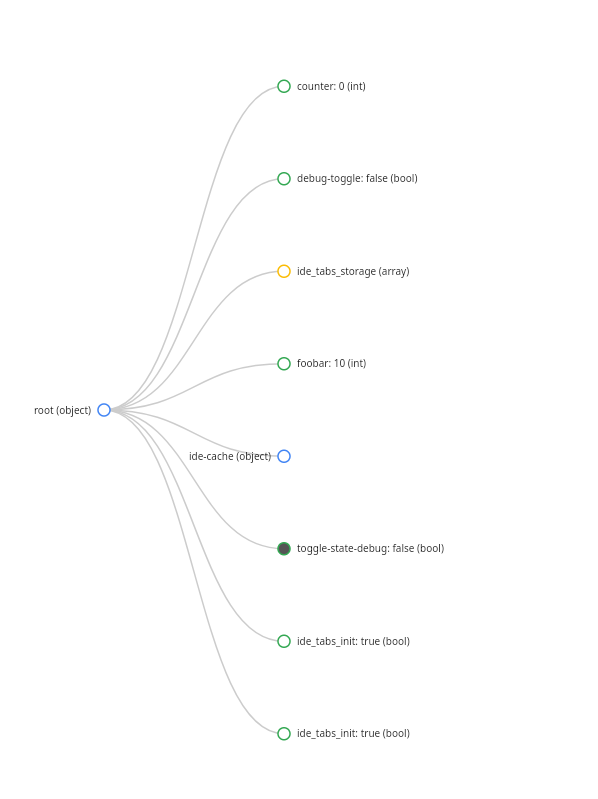
\includegraphics[width=0.75\textwidth]{debug-state.png}
  \caption{
    Module that creates a visualization of the current \gls*{ide} state. The
    visualization is made using an external JavaScript library.
  }
  \label{pic:debugState}
\end{figure}


\subsection{Module Dependency Visualization}

When developing against a modular architecture, it is useful to be able to see
what different module families appear, and what the different dependencies
between the modules are. In picture \ref{pic:modDep} we can see the resulting
graph of the \gls*{ide} modules.

\begin{figure}[H]
  \centering
  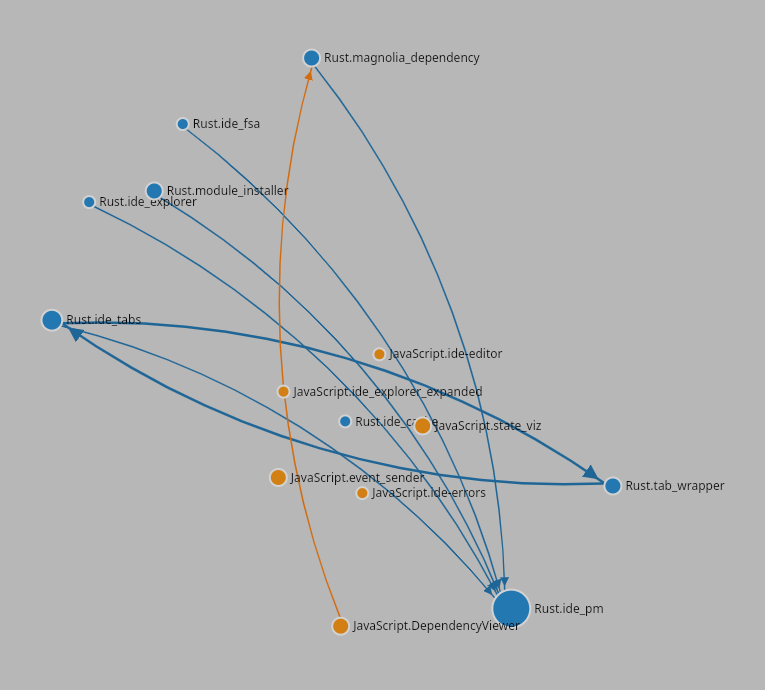
\includegraphics[width=0.75\textwidth]{module-dependencies.png}
  \caption{
    The different modules and their dependencies. Graph was created by using the
    same module shown in picture \ref{pic:magLib}.
  }
  \label{pic:modDep}
\end{figure}


\section{Maintainer}

To make the maintainer of the core application most comfortable, good
documentation is needed. The same documentation a module developer wants, so
it's important for them and the maintainer that the documentation is up-to-date.
But how good is documentation if it is not updated when the code being
documented is changed? This is where Rust's doc-test system comes into play. Any
function annotated with a doc string, can contain code examples. If these code
examples are written as Rust code, and use assert statements, then this code is
run, during testing, as if it was an actual test. Meaning the saying
\textit{code is documentation}, is \textit{documentation is code} in Rust.

\subsection{Testing}

Ensuring the core library used by module developers is correct, is an essential
part of a maintainers job. The easiest way for a maintainer to achieve this, is
to test in production; letting module developers report issues. This is not a
good experience for module developers. But the second-easiest way is to create
unit tests that ensure edge cases are handled correctly. We have designed test
data for serializing and deserializing data between the different languages
supported by the \gls*{ide}, ensuring that any library developed can be
verified to work correctly. The test data is modular, meaning we can easily
create new edge cases. In the picture \ref{pic:libTest}, we can see that there
are $135$ different test cases.

\begin{figure}
  \centering
  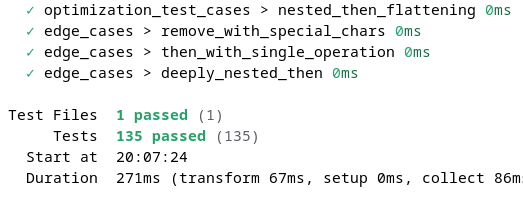
\includegraphics[width=0.50\textwidth]{libtest.png}
  \caption{Picture showing the output of running the test data}
  \label{pic:libTest}
\end{figure}


\chapter{Implementation} \label{cha:impl}

This section will focus on the implementation of the zero core \gls{ide}. In
section \ref{sec:stack}, we will mention technologies used, and why they were
chosen. In section \ref{sec:mod1} and \ref{sec:mod2}, we will discuss the
different iterations the application architecture had, and why they were subpar,
compared to section \ref{sec:moD3}, which is the implementation of the zero core
\gls{ide}. Section \ref{sec:testing} will explain the necessity of testing when
using such a modular design, and explore the ease of which functionality can be
tested.

\section{Tech Stack} \label{sec:stack}

A module can extend an application at either compile time, or during runtime.
This could be achieved by using an interpreted language like JavaScript or
Python. The issue with using a dynamically typed language like Python or
JavaScript, is that it enhances the risk for runtime issues occurring, and when
dealing with scenarios like writing to files, or running long processes like
compiling a program, it is important to avoid such issues. So using a typesafe
language, that can \textit{transform} runtime errors into compile time errors,
is preferred. Furthermore, being able to support runtime modules, in a language
agnostic manner, necessarily means that the core \gls{ide} needs good
\gls{abi} support, and therefore should be implemented in a low level language.
But what does \textit{low level} language mean? And what is an \gls{abi}?

\subsection{Low level languages}

Programming languages has changed over time. In the beginning, a program was a
series of ones and zeros, representing instructions a computer should do. Since
then, we have moved several abstraction layers above what is commonly referred
as \textit{bare metal} programming. From writing in hexadecimal instead of
binary, to machine instructions, to more generic programming language, like C.
What was different with C, compared to writing direct machine instructions, was
that an external program, a compiler, could translate C code to machine
instructions specific to the computers' \gls{cpu} architecture, this meant a
single program, written in C, could be compiled to many different computers. So,
at the time C came out, it was considered a \textit{high level} programming
language, because the language a developer was writing in, had a higher level of
abstraction. Today this notion of \textit{low} and \textit{high} level languages
has changed. A \textit{low level} language is close to how a \gls{cpu}
\textit{thinks}, which has traditionally meant that C is a low level programming
language, but some authors \cite{cNotLowLevel} argue that this is no longer the
case. In any case, we will use \textit{low level} to mean a programming
languages like C, where direct memory manipulations is a feature of the
language.

\subsection{Application Binary Interface (ABI)}

An \gls{abi} is an low-level interface, a kind of \gls{api},
between two programs. Such as C program and its dynamic library dependencies.
The \gls{abi} defines how data is laid out in memory, how functions are
invoked, and other machine level details. Both the C program and the dynamic
libraries must agree on the \gls{abi}, otherwise misinterpreted data or invalid
function calls could lead to \gls{ub}.

\paragraph{Undefined behavior} In programming \gls{ub} occurs when a program
violates the language specification in a manner that is not defined by the
specification. This can be the results of \gls{abi} mismatch, like if the
layout of a struct in memory differs between the parties, in a manner which
leads to breaking of type safety, or direct violations of the language rules,
like null pointer dereference. \gls{ub} is dangerous because the compiler might
optimize the binary unpredictably or the program may behave arbitrary. It is
also a vector of attack for hackers.

\paragraph{Why not C?} C has good parts, like the C-\gls{abi}, which most
languages have bindings too. Using C would mean allowing those languages to
interface with our project, meaning, one step closer to a language agnostic
module architecture. But C has issues, like being the number one cause in
security issues. (This is just because so much of our infrastructure is written
in C, but y'know.) These security issues are mostly caused by memory management.
Would be cool if the C compiler could notify a developer if they were developing
something that could cause an issue in the future. Enter, Rust.

\subsection{Rust}

Rust is a general purpose programming language, designed for, amongst other
things, type safety, memory safety, and concurrency. When programming in Rust,
the bugs common in other languages, like null pointers, buffer overflow and data
races are detected at compile time. Most of these are features of Rusts
ownership rules. These rules, enforced by the compiler, ensure that values are
safely dropped, (freed), this ensures that all variables referenced in Rust have
a value, and can be safely evaluated. It works by simply dropping values when
they are out of scope. The example in listing \ref{lst:ownership}, the
\textbf{name} variable is declared, and used as an argument in the
\textbf{greeting} function. We cannot call the function again with
\textbf{name}, since at the end of \textbf{greeting}, before it returns,
\textbf{name} is dropped, since once we called \textbf{greeting}, the
\textbf{main} method no longer \textit{owned} \textbf{name}, as the ownership
was transferred to \textbf{greeting}. We could \textit{fix} this by changing the
argument type from \textit{name: String}, to \textit{name: \&String}, (commonly
written as \textit{name: \&str}), and adding the borrow symbol to the argument in
the method invocation, as shown in listing \ref{lst:ownership-ref}.

\begin{center}
  \lstinputlisting
    [ language=Rust
    , caption={Ownership example (Rust)}
    , label=lst:ownership
    ]{./code/rust-ownership.rs}
\end{center}

\begin{center}
  \lstinputlisting
    [ language=Rust
    , caption={Ownership example with reference (Rust)}
    , label=lst:ownership-ref
    ]{./code/rust-ownership-ref.rs}
\end{center}

This same principle ensure the other mentioned features of the language,
including performance, as with the borrow checker, there is no need for a
garbage collector. Another Rust feature are so-called \textit{macros}. A macro
is some code that is evaluated and executed at compile time, that may change
the source code. An example of this, can be seen in listing \ref{lst:ownership}.
The \textbf{println!} is a macro invocation. \textbf{println!} is used so that
the developer doesn't have to format the expressions being used, this is handled
by the macro. This is helpful because redundant work can be automated.

Furthermore, Rust has good cross-platform support, ensuring
we can write OS-agnostic code, and compile it to specific targets, without much
hassle. Since Rust is low-level, it has good bindings to C, ensuring
compatibility with future models, made in other languages, by use of the Rust
\gls{abi}.

\subsubsection{Rust Application Binary Interface}

Rust's \gls{abi} is not stable! Because it is not supported by their semantic
versioning. This means even a bug fix in the compiler, could break the
\gls{abi}. So if an application, written in Rust, is compiled in version 1.8.0,
if this application relies on a Rust library that is compiled in version 1.8.0,
everything is okay. But if the application is later recompiled with a compiler
in version 1.8.1, then \textit{undefined} behavior could occur. One of the ways
undefined behavior was avoided, was using the \textit{abi\_stable}-crate, which
enables \textit{safe} loading of external libraries, meaning modules. This is
only an issue for runtime modules, which means they need to be handled
differently than compile time modules.

If the types in the core application change, either by expansion or renaming or
such, the crate would crash the application during startup, because the existing
module would have a different expectation of what types existed, which again,
could lead to undefined behavior. But, this due to the implementation of a
runtime module using the \textit{abi\_stable}-crate, as one could design a
module to be expanded in the future, but due to the stability of the \gls{api},
this was deemed unnecessary.

\subsection{Tauri}

Tauri is a framework for Rust, which enables us to create a cross-platform
application. Any frontend framework that compiles to \gls{html}, JavaScript and
\gls{css} can be used as the \gls{gui}. Such a \gls{gui} is commonly referred to
as a \textit{web view}. This framework also adds support for invoking Rust
methods in the frontend framework, and vice-versa. This allows for support of
JavaScript modules, without much fuzz. Tauri archives with \gls{ipc}, which
allows for isolated processes to communicate securely. For JavaScript to Rust,
this is achieved with something called \textit{Commands}, which acts as an
abstraction on top of the \gls{ipc}, which turns the invocation to a
frontend-backend architecture.

\subsubsection{TypeScript}

Any frontend framework that compiles to \gls{html}, JavaScript and \gls{css} can
be used with Tauri, so TypeScript was chosen. TypeScript offers a lot of
features over JavaScript, amongst them being able to \textit{type} functions,
ensuring null/undefined-safety. Furthermore, by using crates like
\textit{ts-rs}, Rust types can be annotated with attribute macros, which create
a one-to-one mapping between the Rust type, and the serialized JSON object, to
be used in TypeScript, allowing for even more type safety, and ensuring that the
types used in the \gls{ide} only have to be defined one place.

Allowing for any JavaScript library to be used, enabled a low development time
of \gls{ui} components, since this is something that a lot of \gls{ui} and user
experience designers have looked into. So existing code for this already exists
and can be used. \gls{npm}, for example, is a package registry for JavaScript.
It contains around \textit{34 million} libraries, all of which are usable in
this architecture. If the functionality that these libraries are useful for the
application, is another question. This functionality allows for quick
development time for modules, which means features that are standard in
\gls{ide} can be quickly and easily added.

\subsection{Security}

This framework gives a lot of security which is needed in an
application which runs third party code. An example of this, would be the
so-called \textit{isolation pattern} that Tauri supports. Since we allow for
evaluation of JavaScript code in the \gls{ide}, we allow for third-party-code to
access all of Tauris \gls{api}. This \gls{api} is quite powerful, allowing for
features such as access to the system shell, the file system, etc. Being
powerful, it is dangerous to expose this to third-parties, but we can
intercept and modify all Tauri \gls{api} calls sent from the JavaScript side,
before they reach Tauri. We can therefore, depending on the perceived threat or
sensitivity of a Tauri \gls{api} call, choose to disregard the invocation of the
\gls{api}. We could also choose to disregard \textit{all} invocations that comes
from the JavaScript side, effectivaly only allowing Tauri \gls{api} invocations
through the \gls{ide} itself, meaning only Tauri functionality exposed by the
\gls{ide} itself are callable.

This of course has \textit{some} performance implications, as we now have some overhead on
each Tauri \gls{api} invocation, but this is negliable\footnotemark{}

\footnotetext{According to Tauri themself \url{https://v2.tauri.app/concept/inter-process-communication/isolation/\#performance-implications}}

\subsubsection{Module Validation}

Running third-party-code can dangerous. If this code is not validated or does
not come from a trusted source, it could be an attack vector. Luckily, Tauri does
some of this work for us, allowing us to analyze all module to core
communication, but even if we have validated that a module is wanted, there is
still the remaining use that has been the reason for 100\% of all CVE's, human
error.

The Rust compiler can ensure that the Rust modules are valid during compile
time, for runtime this is a bit trickier. But for JavaScript modules, which the
\gls{ide} supports out-of-the-box, this is a bigger issue. This lead to the
development of two systems. \gls{rsms} and \gls{jsms}.

It was necessary to distinguish the different module systems, due to the way
they would be loaded and invoked by the core application. Since the core is
written in Rust, the \gls{rsms} doesn't have to do any validation or
translation when communicating with compile time modules. With runtime modules
this also ended up being trivial, but will be discussed more in depth later.

In the \gls{jsms}, managing of modules can lead to exceptions being thrown.
Since third party code is being run, nothing can be trusted. All module
invocations and outputs needs to be sanitized before it can be used in the core
application. This is achieved by wrapping all invocations in a
\textit{try-catch}, and using the \textit{io-fp} library to decode types during
runtime. This enables us to safely invoke modules, as we can translate all
computations into a product type, where it is either a success, giving us the
wanted computation from the module, or an error. But even with types, we cannot
verify functions. Since during runtime, we are in the JavaScript environment,
we can only validate if something is a function, using the
\lstinline[language=JavaScript]{typeof} operator. It is possible to do
\textit{some} verification on functions in JavaScript, but this is only a) Is it
a function, and b) does it have the correct amount of arguments. In this case,
one. Nothing about the typing of the function can be ascertained at runtime,
without explicitly invoking the function.

\section{Module V.1} \label{sec:mod1}

We did not attempt at first, to create a zero core application; this was a
\textit{natural} conclusion to the existing problem. The first attempt was a
simple generic \gls{ide}, in which the module architecture was a concern from
day one of development. The general plan was this:

\begin{enumerate}
  \item Create an \gls{ide}
  \item Extend the \gls{ide}, to allow for a module architecture
  \item Modules call the application using some DSL
\end{enumerate}

Since any JavaScript frontend framework could be used, React was chosen, one of
the reason for this choice was due to its popularity, which again, would speed
up the development time of the application, but also due to the way React
renders the \gls{html}. Between two different re-renders of the application,
React can check the difference between the \gls{vdom}, which is React's
representation of the \gls{dom}. It then only changes what is needed in the
\gls{dom}, instead of re-creating the entire \gls{dom}, which makes the render
time quick.

This was the more straight forward way to work, because as we could model it of
existing \gls{ide}s, like \textit{Visual Studio Code} or \textit{Eclipse}.
Another advantage is that when implementing the application, one necessarily
gets a better understand of how eventual modules should extend the application.

This approach did unfortunately not lead to a truly modular application. Similar
issues to existing \gls{ide}s, how does one allow for \textit{everything}?
Furthermore, anything created this way, would be subpar to existing software,
which would lead to the next maintainer having to fix the core application. This
in turn, would add a lot of complexity, which the maintainers would have to deal with.

\section{Module V.2} \label{sec:mod2}

\begin{enumerate}
  \item Everything is a module
\end{enumerate}

Instead of developing features that make up an \gls{ide}, and attempting to
ensure it is implemented in such a manner that it can be modified in the future,
make everything modular. The only thing the \gls{ide} can do, is to manage
modules. All features, from the file explorer to the text editor, everything is
a module that can be enabled or disabled.

\subsection{The Elm Architecture}

An inspiration for the new module architecture is Elm-Lang \cite{elmLang}. Elm
is a functional language, aimed at frontend web development, but its
architecture is quite interesting. As one can see in figure
\ref{fig:elmArchitecture}, is used by the Elm-runtime, which translates the Elm
code into \gls{dom} manipulations, and translates \gls{dom} events into
\textit{Msg} which is handled by the Elm code. This was the inspiration for the
new module architecture. A module is managed by the runtime, which is the
\textit{core} application. But with some inspiration from \gls{mvc}, where
instead of the module keeping its own state, this is again managed by the core,
allowing for multiple modules to read and react to states updated by other
modules, allowing for more interactivity between modules, and therefore being
more modular.

\begin{figure}
  \centering
  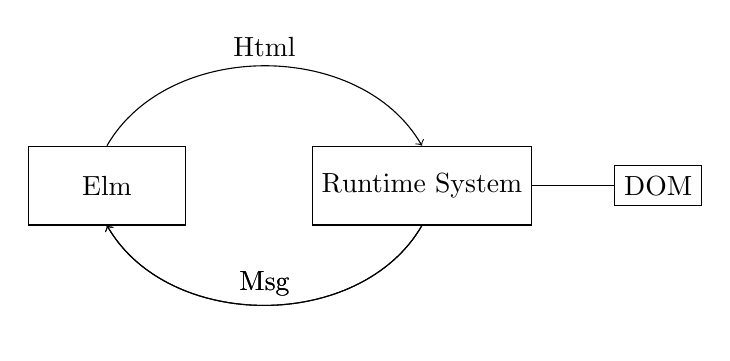
\begin{tikzpicture}
  % Nodes
  \node (p) [rectangle, draw, minimum height=1cm, minimum width=2cm] at (0, 0) {Elm};
  \node (i) [rectangle, draw, minimum height=1cm, minimum width=2cm] at (4, 0) {Runtime System};
  \node (d) [rectangle, draw, minimum height=0.5cm, minimum width=1cm] at (7, 0) {DOM};
  % Arrow
  \draw[->] (p.north) to[out=60, in=120] node[midway, above] {Html} (i.north);
  \draw[->] (i.south) to[out=-120, in=-60] node[midway, above] {Msg} (p.south);
  \draw[->] (i.south) to[out=-120, in=-60] node[midway, above] {Msg} (p.south);
  \draw[] (i) -- (d) node[midway, above] {};
  % Header
\end{tikzpicture}

  \caption{Elm Architecture (Figure adapted from \cite{elmFig})}
  \label{fig:elmArchitecture}
\end{figure}

\subsection{Module Architecture}

In this application, the Elm-box is a module, while the runtime system, is the
core itself. The core invokes all modules, all of which, should have these three
functions, \lstinline{init}, \lstinline{update}, and \lstinline{view}.

\paragraph{Init} Returns a collection of key-value-pairs, which represent
the state of the core.

\paragraph{Update} Returns a collection of key-value-pairs, which
overwrite existing key-value-pairs in the state, or are appended to the state.
Invoked every time a \textit{Msg} is sent.

\paragraph{View} Returns a collection which represents \gls{html},
which is rendered by the core.

A module is initialized by invoking the \textbf{init} method, which returns a
state. This can be seen in figure \ref{fig:moduleInit}. After the state
initialization, the modules' \textbf{view} method is invoked, which initializes
the \gls{ui} for the user, which can be seen in figure \ref{fig:moduleInitView}.

\begin{figure}
  \centering
  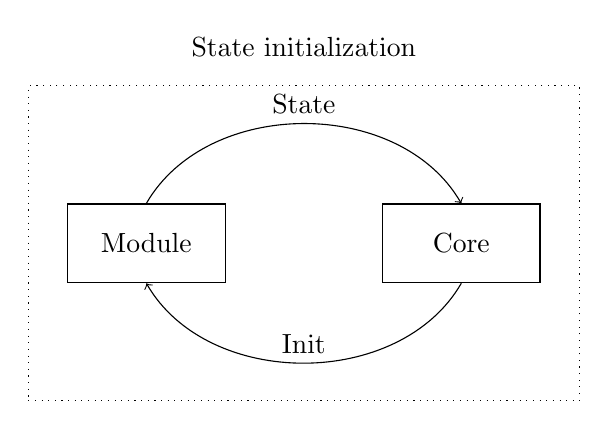
\begin{tikzpicture}
  \node [rectangle, draw, minimum height=4cm, minimum width=7cm, dotted] at (2, 0) {};
  \node [] at (2, 2.5) {State initialization};

  \node (i) [rectangle, draw, minimum height=1cm, minimum width=2cm] at (4, 0) {Core};
  \node (p) [rectangle, draw, minimum height=1cm, minimum width=2cm] at (0, 0) {Module};
  \draw[->] (p.north) to[out=60, in=120] node[midway, above] {State} (i.north);
  \draw[->] (i.south) to[out=-120, in=-60] node[midway, above] {Init} (p.south);
\end{tikzpicture}

  \caption{Module state initialization stage}
  \label{fig:moduleInit}
\end{figure}

\begin{figure}
  \centering
  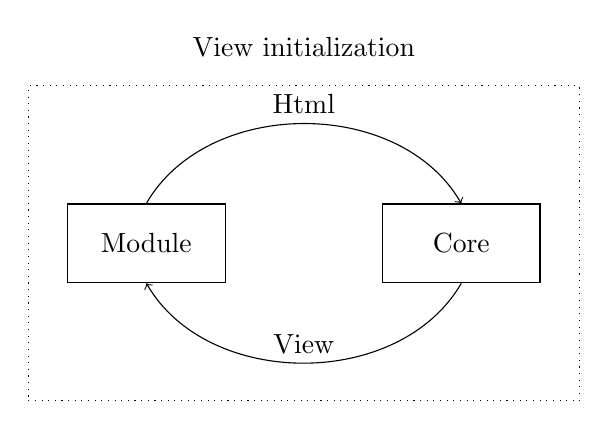
\begin{tikzpicture}
  \node [rectangle, draw, minimum height=4cm, minimum width=7cm, dotted] at (2, 0) {};
  \node [] at (2, 2.5) {View initialization};

  \node (i) [rectangle, draw, minimum height=1cm, minimum width=2cm] at (4, 0) {Core};
  \node (p) [rectangle, draw, minimum height=1cm, minimum width=2cm] at (0, 0) {Module};
  \draw[->] (p.north) to[out=60, in=120] node[midway, above] {Html} (i.north);
  \draw[->] (i.south) to[out=-120, in=-60] node[midway, above] {View} (p.south);
\end{tikzpicture}

  \caption{Module view initialization stage}
  \label{fig:moduleInitView}
\end{figure}

Since the \gls{ide} is written in both TypeScript and Rust, a method of encoding
type information when crossing between the TypeScript and Rust environment was
needed. It was achieved by simply typing \gls{json} objects, so while the state
could be represented as any \gls{json} object, it was instead represented as
nested \gls{json} objects, where, all values, except \textbf{null}, where
encoded as an object with one field, being the type of the object, and then the
value. So an int would be \textbf{\{ int: 0 \}}.

The reason for representing a JSON object as key-value pairs, is that this could
be easily translated to a Rust representation of the same type, using the
\textit{Serde} crate. This allows for creating Rust structs which represents
JSON objects, and creates an automatic encoder/decoder between Rust and
\gls{json}. Using the \textit{ts\_rs}, we could also automatically create the
TypeScript type that represents the automatically encoded/decoded \gls{json}.
This ensures a good cooperation between the \textit{frontend} and
\textit{backend}.

\subsection{IDE lifecycle}

The general idea was that for each possible \gls{dom}-event, there would exist a
way to send a Msg. Each Msg contains a Msg name, and some value, which enabled
pattern matching on Msg, similar to Elm, for modules, so each module could
choose to act on a Msg or not. So, after the initialization of the \gls{ide},
any time the user interacted with the \gls{gui} the modules would react to the
Msg. The trivial plugin, would simply return an empty state on \textbf{init} and
\textbf{update}, while on \textbf{view}, it would return a \textit{frag}
element, which is a React element that evaluates to no \gls{dom} change.

In listing \ref{lst:pluginCounterExample}, an example of a counter module can be
seen. This module initializes a state, containing the field \textbf{"counter"},
with the value \textbf{VInt 0}.

The \textit{update} function the module exposes, matches on a \textbf{"counter"}
msg, with a \textbf{VInt i} value. If the given Msg matches this, then the
module adds to the \textbf{"counter"}-field, the value from the Msg, which is
$1$.

Finally, the \textit{view} function renders a button, which when pushed by a
user, sends the \textit{counter-Msg}.

\begin{center}
  \lstinputlisting
    [ language=Haskell
    , caption={Counter Module (Haskell)}
    , label=lst:pluginCounterExample]{./code/plugin-counter-example.hs}
\end{center}

\subsubsection{Module purity}

One important thing in this architecture, is the pureness of module. The state
of a module needs to be kept in the core application, and not in the module
itself. The reason for this is twofold. It allows for the possibility of the
core to be optimized in the future, as modules which do not react to a certain
msg-state combination, can be noticed, and ensure modules are not unnecessarily
invoked. It also lowers the complexity for module developers, as it is easier to
reason about modules if \textit{all} they do is read or write to some state.

If we have the modules $A$ and $B$, where their relationship is $A \to B$,
meaning $A$ \textit{invokes} $B$ by sending some Msg, which $B$ reacts too, and
we want something to happen before $B$ reacts, we can add a new module, $C$,
which also reacts to the same Msg, but if we know the name of the module $B$,
we can set the name of module $C$ to be \textit{above} the order, relative to
$B$, ensuring that $C$ always triggers before $B$.

\subsection{Module v2 Cons}

\paragraph{Not modular} This setup is also not really modular, as a single
module cannot invoke another module without being impure. The only way to
invoke/trigger another module, is to throw a \textit{Msg}, which would trigger
an update -> view -> cycle. So a module cannot \textit{listen} for a single
message, all modules are triggered by the same \textit{Msg}, and handled
accordingly, synchronously.

\paragraph{Synchronous Module Invocation} If a Msg triggers a computational
heavy method, the \gls{ide} will \textit{hang}, and act \textit{sluggish} until
the computation has finished. This would also affect \textit{all} modules,
since they are invoked in order, regardless of if they actually change the
state or view.

\paragraph{Ever-growing State} There was no way to remove a field on the state,
the state is appending/overwriting -only, which was a side effect of the
\textit{solution} to state collisions.

\subsubsection{State Collision} \label{sec:collision}

A state collision occurs when two or more modules updates the same field, during
the same update-cycle. This issue also occurs when folding two states. After any
update-cycle, we were left with a list of states, which needed to be coalesced
into a singular one. There are several different ways to correct a collision
between two states:

\begin{enumerate}
  \item If the states are of same type:
    \begin{enumerate}
      \item If the value from one of the colliders are unchanged from the previous state:
        \begin{enumerate}
          \item Keep the new value OR Keep the old value
        \end{enumerate}
      \item Else
        \begin{enumerate}
          \item Apply the types' semigroup operator to the fields.
        \end{enumerate}
    \end{enumerate}
  \item Else
    \begin{enumerate}
      \item If the value from one of the colliders are unchanged from the previous state:
        \begin{enumerate}
          \item Keep the new value OR Keep the old value
        \end{enumerate}
      \item Else
        \begin{enumerate}
          \item Keep the left-hand side value OR Keep the right-hand side value
        \end{enumerate}
    \end{enumerate}
\end{enumerate}

Since the states are ordered by the name of the module they come from, we
have a consistent ordering of left-hand side and right-hand side. Due to the
fact that module invocation is synchronous, and ordered. If the same modules
gives a collision on the same input, (given that all modules are pure), the
resulting state will be the same every time. The problem is that applying some
function on the values could be an unwanted way to resolve collisions. The
standard way will be to log the collision, and then drop both states. Even
if two states have $A$ and $B$ amount of fields, and just one collision, we will
drop $A + B$ amount of fields.

This problem of resolving state collision only occurs because each module
returns a subtree of the state. We then have to analyze the new coalesced tree
for each new subtree that is added, to figure out if there occurs any collision.
And then notifying the module developer of which field this collision occurred
on, and which modules tried to modify that field.

\section{Module V.3} \label{sec:moD3}

The third and hopefully final, plan:

\begin{enumerate}
  \item Everything is a module
  \item Modules can \textit{invoke} modules
\end{enumerate}

A module only exposes two functions:

\paragraph{Init} Returns nothing

\paragraph{Handler} Returns nothing

In the previous architecture version, each module directly changed the state,
which caused issues. Instead, each modification a module does, \textit{acts}, as
a direct modification, but is in fact, translated to a DSL which can be analyzed
for possible collisions. This was discovered to be a need, as in the new
version, the \gls{ui} was also restructured, to allow for less re-rendering, and
this restructuring, made it clear that changing the state, or changing the
\gls{ui} is just tree manipulations, which will be discussed more later.

\subsection{Zero core architecture and microservice architecture}

The new plan came with a change of viewpoint. Think of
\textit{everything being a module}, this pushed for a modularization between the
then tightly coupled parts, the \textit{frontend} and \textit{backend}. As
mentioned, having two different languages could allow for easier support of
modules written in different programming languages, but for this to work in an
optimal way, both the \textit{frontend} and \textit{backend} should be loosely
coupled. This is an equivalent architecture to microservices.
\todo{Add diagrams and examples}

\subsection{Vanilla TypeScript}

Instead of using React as the frontend framework, TypeScript was chosen, which
simplified the integration between the backend and frontend, as the complexity
of React's state management could be avoided, along with React's hydration.
Given the rendering was now more \textit{hands-on}, the core could expose a lot
of the functionality for rendering, which modules could change. This would
increase the difference between the \gls{jsms} and \gls{rsms}, as the backend
was not privy to this API, but this was not seen as an issue, as this API would
turn module non-pure.

\subsubsection{Removing abstractions}

It became prudent, due to the change of architecture, to change the entire
frontend, moving away from React, and using \textit{bare-bones} TypeScript. This
would enable easier integration into the \gls{jsms}.

\subsection{Core Modifications}

Learning from the issues outlined in section \ref{sec:collision}, instead of a
module returning the new core, it will rather return a set of instruction on
\textit{how} the core is to be modified, resulting in what the module developer
wants the core to be. The reason for turning it around in this manner, is that,
the new architectural change also came with a change on how the \gls{ui} is
modeled, as it is now up to the core to figure out an inexpensive way to do
rendering. Since the core has \gls{ui}-structure which is a representation of
what the \gls{dom} should be, it can be treated as a Virtual-\gls{dom}, similar
as to how React does it. This also means that there could be a collision on
\gls{ui}-change, as well as on a state-change. Instead of solving the equivalent
problems twice, it was decided to try to treat the issues with collisions in
state and \gls{ui} as the same issue; its some form of tree-manipulation. We
could then reduce the amount of needed methods on the module instance, to two.
One for initializing the state, and one for handling events. In \ref{lst:cm},
we have a \textbf{CoreModification} type, which has two fields, one for the
state, and one for the \gls{ui}.

\begin{center}
  \lstinputlisting
    [ language=Rust
    , caption={Core Modifications (Rust)}
    , label=lst:cm
    , firstline=12
    ]{./core/src-tauri/core-std-lib/src/core_modification/mod.rs}
\end{center}

\subsection{Tree Manipulation}

This restructure changes the way the view is rendered. Instead of the view being
re-rendered for each state-update, the view, or \gls{ui}-hierarchy, is only
modified by modules. This modification is similar to the earlier state
modification, so a unified algorithm to solve this can be used. If there is an
easy way to translate a \gls{ui} modification to a state modification, and back
again. To solve this, instead of having a module return the actual
modifications, meaning, the updated core, a module returns a set of instructions
of what to do with the core.

\begin{center}
  \lstinputlisting
   [ language=Rust
   , caption={Instruction (Rust)}
   , label=lst:inst
   , firstline=6
   , lastline=16
   ]{./core/src-tauri/core-std-lib/src/instruction/inst.rs}
\end{center}

In the listing \ref{lst:inst}, it is clear how the \textbf{Instruction}-set makes the
modification of the core, a kind of group, as given by the definition
\ref{def:group}. Intuitively, for any \textbf{Instruction}, there exists
an \textit{inverse} one, such that the definition \ref{def:inv} is upheld. If we
add some value to the state, we can find an remove instruction that removes
that field from the state, as shown in listing \ref{lst:inst}, in the
\textbf{combine} method.

\begin{remark}
  The \textbf{combine} method does not recursively check the \textbf{Then}
  instruction for \textbf{Instruction}s that lead to a \textbf{NoOp}, but in the
  core \gls{ide}, there is an optimization step that does this.
\end{remark}

To formalize this, that the \textbf{Instruction}-set is an group, we can look at
a subset, since \textbf{Instruction} is parameterized by some type \textbf{T},
we will look at it when \textbf{T} is \textbf{Value}, noted by the subscript
\textbf{val}.

\begin{theorem}[Instruction Group] \label{thm:intr}
  Let $\Sigma$ be the set of all strings, $Val$ be the set of all
  \textbf{Values}, $Html$ be the set of all \textbf{Html} variants, and
  $Inst_{val}$ be the set of all \textbf{Instruction} defined as:
  $$
    NoOp = \left \{ noOp \right \}
  $$
  $$
    NoOp \in Inst_{val}
  $$
  $$
    Add_{val} = \left \{ (x, y, z) \vert x \in \Sigma, y \in \Sigma, z \in Val \right \}
  $$
  $$
    Add_{val} \in Inst_{val}
  $$
  $$
    Rem_{val} = \left \{ (x, y, z) \vert x \in \Sigma, y \in \Sigma, z \in Val \right \}
  $$
  $$
    Rem_{val} \in Inst_{val}
  $$
  $$
    Then_{val} = \left \{ (x, y) \vert x, y \in Inst_{val} \right \}
  $$
  $$
    Then_{val} \in Inst_{val}
  $$
  For any $x \in Add_{val}$ there exist a unique $y \in Rem_{val}$, such that:
  $$
    x \oplus y = noOp
  $$
\end{theorem}

The theorem \ref{thm:intr}, unfortunately, cannot be encoded in Rusts type
system, but when implementing $combine$, we can map the variants along with the
specific fields being added ($Add$), modified ($Mod$), or removed ($Rem$), to get
a more optimized instruction set. If we are modifying a value on field $foobar$,
but in the same instruction set, remove it, then the modifying instruction is an
$NoOp$. This optimization can be found in appendix \ref{app:a}.

Like writing direct binary to develop a program, writing \textbf{instruction}s to
change the core is quite abstract for most developers so to facilitate development
of modules, a helper class was created, which \textit{translates} modifications
to instructions. As shown in listing \ref{lst:ui-builder} and
\ref{lst:state-builder}, a module developer simply invokes different methods on
the builder, eventually building a \textbf{CoreModification}, to be sent.

\begin{center}
  \lstinputlisting
   [ language=Rust
   , caption={
     UI Builder (Rust) showcasing how to add an empty \gls{html} div element to
     the root \gls{html} element.
   }
   , label=lst:ui-builder
   ]{./code/module-ui-builder.rs}
\end{center}

\begin{center}
  \lstinputlisting
   [ language=Rust
   , caption={
     State Builder (Rust) showcasing how to add a \textit{count} field to the
     state, also showcasing how Rust can infer that the i32 type $0$ is
     a \textbf{Value::Int} type.
   }
   , label=lst:state-builder
   ]{./code/module-state-builder.rs}
\end{center}

This allows for an ergonomic way for module developer to create modifications on
the core, without having to understand the syntax of the
\textbf{Instruction}-set.

\subsection{Backend Agnostic Frontend}

Since we are using the framework Tauri to implement the \gls{ide}, the \gls{ide}
is split to two, loosely coupled parts. The \textit{frontend} and
\textit{backend}. The frontend acts as a thin wrapper around the core \gls{api},
enabling different \textit{runtimes} to handle module management, while the
frontend waits for events, and renders the \gls{gui}. This structure allows for
future maintainers of the \gls{ide} to be able to \textit{trivially} switch
runtime, if they wanted to use some other language to implement the runtime
system in, like PureScript, Gleam or Haskell, all of which can target
JavaScript, then they could.

\subsection{Making the Core evaluate modifications asynchronously}

Due to Rust first class focus on concurrency, it was trivial to make the core
modifications run asynchronously. In previous iterations, the core evaluated
one event at a time, waiting until all modules had finished their computations,
before emulating the change and allowing for the next event to be evaluated. But
this caused a noticeable \textit{lag} if an event was long. This was solved by
changing the core modification evaluation from a simple method to be invoked, to
an \gls{mpsc} channel system. Using \textit{tokio}, a Rust crate for
asynchronous development, a channel for core modifications was created, and
instead of the core collecting all modifications, each module is invoked and
\textit{awaited} for in a separate thread, where in each module, if they have a
core modification, sends the modification to the core channel, which works on
a first come, first server basis. Here the core can evaluate the changes, also
on a separate thread.

\section{Testing} \label{sec:testing}

A zero-core \gls{ide} is equivalent to a microservice architecture, in that
testing is important to ensure changes in one module does not inadvertently
affect another. This is commonly achieved by using \textit{pipelines}, a part
of the \gls{cicd} process, where we run several \textit{jobs} whenever we make a
change to our application. If we are bundling different modules together, and
serving that as an \gls{ide}, we want to ensure that a change to a module does
not negatively affect the other. This is where \textit{pipeline jobs} come in,
as each \textit{job} test some part of our \gls{ide}. While it is cheaper to
\textit{spin} up an instance of the \gls{ide} in a pipeline, than an application
dedicated to serve millions of users, we still want to avoid doing this
unnecessarily. This is why we split up our testing into different stages.

\subsection{Mocking}

Due to the \textit{pureness} of modules, mocking can be achieved easily, and
therefore, modules can be tested alone, which is good, because testing a
singular module is inexpensive. There are several ways to do this mocking in our
architectural setup. For both the \gls{jsms} and \gls{rsms}, there are
\textit{mock-cores}, which can mock the expected functionality of the Core
instance, which we can extend to evaluate actual modifications, ensuring we can
assert that some state or \gls{ui} change has occurred after an Event has been
sent.

\subsection{Unit Testing}

A module developer should create unit tests for their module. This can easily be
done, and tested many times, due to the light-weightiness of a module. This,
together with mocking, ensures we can test our modules, as if they were in a
\gls{ide}. Which means we can ensure changes made to a module is non-breaking.

This also applies to maintainers of the \gls{ide}, as maintaining the core
functionality and \gls{api} of our library, means documenting possible breaking
changes, which unit tests can help ensure.

\subsubsection{UI Testing}

We can also combine this with existing testing libraries, like \textit{Playwright}\footnote{\url{https://playwright.dev/}},
which can enable us to create tests specifically for UI behavior. In the case of
\textit{Playwright}, our \gls{ui} testing is dependent on that our
\textit{mock-core} has the necessary functionality to transform the
\textbf{Html} type we have implemented, to actual \gls{html}, which can be
rendered on a webpage, or \textit{headless}, in \textit{Playwright}s case, so
that \textit{Playwright} can assert the state of our \gls{dom}.

\subsection{Module Family Testing}

If a module changes some feature, let's say in the editor functionality, the
module family tree encompassing this functionality needs to be tested, to ensure
nothing breaks. This means creating tests that use all the modules in a family,
and asserting that the state and \gls{ui} behave as expected. In the case of
the editor functionality, that after the Event \textit{open-file} is sent with
a path to some file, that there exists a \textit{textarea}-\gls{html}-element in
the \gls{dom}, with the same contents as the file.

\subsubsection{Contract Testing}

As a module developer, on is designing some kind of \gls{api}, but the developer
has no say in how a consumer of the \gls{api} consumes it. In a microservice
architecture, the common way to work around this, is to version control the
\gls{api} by prefixing \textit{v*} in front of all endpoints in the \gls{api},
where star, (*), is the version of the \gls{api}. This way, the \gls{api}
designer can develop new \gls{api}s, without worrying about breaking
functionality that consumers of the \gls{api} depend on. This, however, usually
means having to maintain equivalent \gls{api}s in parallel, until one decides
to deprecate an older less used version, forcing consumers to move on to the
newer version of the \gls{api}.

Instead of relying on such a versioning system, module developers could use
\textit{contract testing}.

\paragraph{Contract Testing} Imagine some \gls{api}, and several consumers,
$A, B, C$, The \gls{api} developer is serving some data, in this case an
integer number, which all the consumers use. One day, the developer finds out
that using integers is not optimal, and want to move on to using floating point
numbers instead. Changing the \gls{api} outright could bring issues, as the
consumers might rely on the \gls{api} being an integer, instead of a float. But
the change is needed, or wanted, at least. In this scenario, it is \textit{easy}
to inform all the consumers of the \gls{api}, but if the consumer count
increases tenfold, this is more difficult. A notice can still be sent, but it is
not feasible to ensure all consumers commit time to change their ways. Contract
testing ensures that, if a change like this occurs, the maintainer of the
\gls{api} is notified by which consumer this change breaks.

The issue is to create these contracts. Using frameworks like Pact \cite{pact},
a developer creates a \gls{dsl} test, where they describe how the provider or
consumer reacts to certain interactions. But since everything is a module, we
can automate this.

\subsection{Automating Contract Testing}

This process could be partially automated, as all modules have to register the
event they want to handle. Furthermore, all events thrown are also explicitly
done through the core instance, meaning a \textit{test-core} could be created,
which registers which event is thrown from what module, and all dependencies
between modules can be noted.

\subsection{End-To-End-Testing}

The final step in the testing pipeline, is to test the entire application
together. This is known as \gls{e2e}. \gls{e2e} is expensive, compared to the
other steps, as we have to load the entire application in the pipeline, and test
all interactions. This, of course, is the easiet way to cover all edge-cases, but
since it is the whole application being tested, harder to figure out what caused
a failure. Our \gls{ide} can be saturated with events in the \gls{e2e} step of a
pipeline, as all user interactions are translated into events, this ensures a
module developer can narrow down what modules are at fault, by what modules
\textit{subscribe} to that event.

\section{Module Developer Tools}

The module developer experience is an important aspect of a zero-core
architecture. A good way to improve this experience, is by providing good
tooling.

\subsection{Module Dependency Visualization}

\todo{Still being developed}

\subsection{Module Isolation Testing}

\todo{Still being developed}

This is as simple as creating a minified version of our \gls{ide}, that has
extra tools for mocking Events.

\subsection{Module Boilerplate Generation}

\todo{Still being developed}

This \gls{cli}-tool enables a developer to quickly get started on developing
modules, as the tidous work of setting up a project can be automated away.

\section{Modules}

\paragraph{Event Type} In listing \ref{lst:moduleEvent}, one can see the
structure of an event type. This allows for modules to pattern match on specific
events, and unlike, as in the previous version, modules can \textit{subscribe}
to specific events to react to. This changes the structure of the module
architecture to go from one wherein the core is a terminal object, to a more
\textit{complicated} one, in which module families can form.

\begin{center}
  \lstinputlisting
    [ language=Rust
    , caption={Module Event (Rust)}
    , label=lst:moduleEvent
    , firstline=14
    , lastline=41
    ]{./core/src-tauri/core-std-lib/src/event/mod.rs}
\end{center}

This forms our \textit{request} and \textit{response} type, making the
equivalence with a \gls{rest} \gls{api} obvious. The clients and consumers
of the \gls{api}, are the modules which can be seen in listing \ref{lst:mod}.

\begin{center}
  \lstinputlisting
    [ language=Rust
    , caption={Module trait (Rust)}
    , label=lst:mod
    , firstline=12
    , lastline=16
    ]{./core/src-tauri/core-module-lib/src/lib.rs}
\end{center}

A module can interact with the core, by getting the state, \gls{ui},
\textit{throwing} an event, registration themselves to \textit{handle} an
event, or to \textit{send} a \textbf{CoreModification}. In listing
\ref{lst:core}, we can see this core trait.

\begin{center}
  \lstinputlisting
    [ language=Rust
    , caption={Core trait (Rust)}
    , label=lst:core
    , firstline=6
    , lastline=18
    ]{./core/src-tauri/core-std-lib/src/core.rs}
\end{center}

Since a module updates the core by \textit{choosing} to send a
\textbf{CoreModification}, through a \gls{mpsc}-channel, a module can run an
expensive computation on another thread, while \textit{ending} their
invocation, ensuring a smooth \gls{ide} experience.

Here are some examples of modules implemented using the proposed architecture.


\subsection{Module Tools}

When developing against a module architecture, having tools to help debug issues
is useful. \dots

Some examples of issues we have experienced when developing modules are as
follows:

\begin{enumerate}
  \item Incorrect handler registration
  \item Incorrect Event name
  \item Incorrect arguments in response
  \item Incorrect arguments in request
  \item Incorrect State
  \item Concurrent Events
\end{enumerate}

Most of these issues relate to the Event system, so being able to mock events
is a useful tool. Luckily, this is quite simple to implement. In
picture \ref{pic:eventMock} we can see this in action.

\begin{figure}[H]
  \centering
  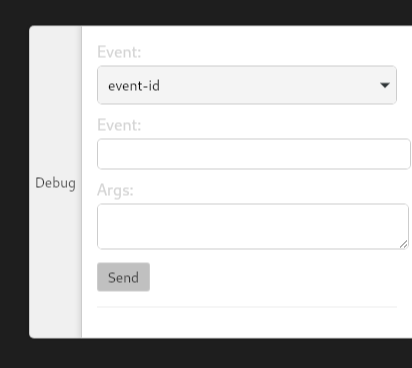
\includegraphics[width=0.75\textwidth]{event-mocking.png}
  \caption{
    Event Mocking module that adds a simple pop-up menu for manually sending
    Events, with specific arguments
  }
  \label{pic:eventMock}
\end{figure}

When mocking in \gls{rest}-\gls{api} development, one creates the expected
response, which is usually a \gls{json}-file. The same is done here, where the
\textit{Args} field in this form expects the argument to be in \gls{json}. This
is helpful, as other testing libraries, like \textit{Playwright} does the same,
and the \gls{ide} logs the Event arguments in the same formatting, meaning we
can simply copy-paste the Event argument we want to mock, into the field.

In the picture \ref{pic:debugState}, we can see a module which helps visualize
the current state of the \gls{ide}, in a tree-graph.

\begin{figure}[H]
  \centering
  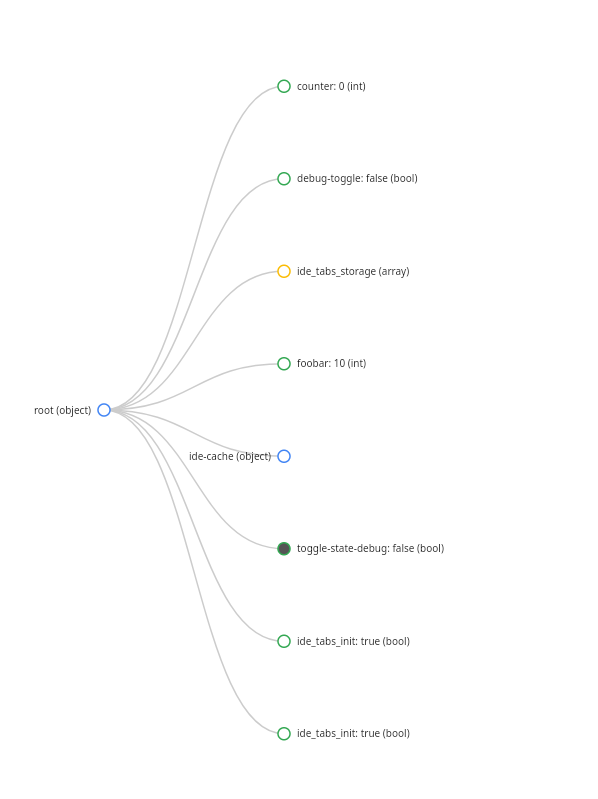
\includegraphics[width=0.75\textwidth]{debug-state.png}
  \caption{
    Debug-tool for visualizing the current \gls{ide}-state
  }
  \label{pic:debugState}
\end{figure}

\subsection{Module Installer}

Module markets are an important part of the \gls{ide} user experience. Being
able to install a module with the click of a button essential. Not having a
dedicated module market like \gls{vscode}, has not been detrimental for
\gls{vim}, as with a \textit{plugin manager}, a user can install a module by
simply supplying a URL to a GitHub repository. Similarly, we allow users to
either install modules from disk, or by supplying a URL to a GitHub repository.
In the picture \ref{pic:moduleInstaller}, we can see such a form. A user can
either install a module from disk, in which case, we simply copy the module
binary at the given path to the runtime module folder, or if a URL has been
supplied, we get the latest released binary from that GitHub repository, and
copy this binary instead.

\begin{figure}
  \centering
  
\includegraphics[width=0.50\textwidth]{module-installer.png}
  \caption{
    A module installation form, where a user can supply a path to a module on
    disk, or a URL to a GitHub repository containing the module binary.
  }
  \label{pic:moduleInstaller}
\end{figure}

\subsection{Magnolia Dependency Graph Visualizer}

In Magnolia, as in many other languages, one cannot have a cyclic dependency.
This means that the dependency graph of a Magnolia project should be a
\gls{dag}. And since Magnolia has such a focus on reuse, the dependency graphs
in a Magnolia project could be quite large. Which means the cycles could be
quite long, which would make resolving the cyclic dependency issue complicated.
One way to help a developer, would be to give them a tool to visualize the
dependency graph, so that they could see what modules are connected. Using the
Magnolia library as the input, we can create a visualization of the dependencies
in Magnolia. Using two modules, one for \textit{parsing} the Magnolia library,
finding all packages, and their dependencies, and another for visualizing
this.

\begin{center}
  \lstinputlisting
    [ language=Rust
    , caption={
      Magnolia library parser Module \textit{subscribing} to an
      \textit{get\_magnolia\_graph } Event (Rust)
    }
    , label=lst:magnoliaLibParserSub
    , firstline=33
    , lastline=36
    ]{./modules/magnolia\_dependency/src/lib.rs}
\end{center}

In listing \ref{lst:magnoliaLibParserSub}, the module is invoking the
\textit{add\_handler} method on an object that implements the \textit{Core} trait,
(\ref{lst:core}), and passing \textit{get\_magnolia\_graph} and
\textit{MODULE\_NAME}. This means that Events with the event name
\textit{get\_magnolia\_graph}, will trigger this module. It's \textit{this}
module, because we have to pass the name of the module handling the event.

We can therefore invoke this Module by simply triggering the subscribed Event.

Due to Rust's type safety, there is a lot of \textit{noise}, especially because
we are working with recursive data structures, with optional values. In listing
\ref{lst:magLibParserSimple}, we can see a simplified version of the module
handler, but this is not valid Rust code, the full code for the module can be
found in appendix \ref{apx:b}.

\begin{code}[H]
  \lstinputlisting
    [ language=Rust
    , caption={Simplified magnolia library parser Module (Rust)}
    , label=lst:magLibParserSimple
    , numbers=left
    , numberstyle=\tiny\color{gray}
    ]{./code/mag\_lib\_simple.rs}
\end{code}

The above code (\ref{lst:magLibParserSimple}), we are handling Events with the name
\textit{get\_magnolia\_graph}, (line 3), and getting the path that is supplied in
the Event argument, (line 4). In line 4 we then create a \textit{key}, which we
use to check if this graph has been created yet, by checking the state (line 6).
If this graph does exist, we \textit{respond} by throwing an Event with the
existing graph (line 7 to 9). If it does not exist, we create it by calling the
\textit{get\_graph} function, (left out for brevity), which recursively finds
files in the supplied path, using RegEx to find the packages, and their
dependencies. We then end by \textit{responding} with the created graph,
(line 12), and store it in the state, with the key (line 13 to 16). The
resulting response can be seen in listing \ref{lst:magLibParserRes}

\begin{code}[H]
  \begin{lstlisting}[
      language=TypeScript
    , label=lst:magLibParserRes
    , caption={Magnolia library parser response (TypeScript)}]
    {
      event: {
        event: "graph",
        args: {
          list: [
            {
              obj {
                name: { str: string },
                dependencies: { list: [{ str: string }] }
              }
            }
          ]
        }
      }
    }
  \end{lstlisting}
\end{code}

The module responsible for rendering the graph, uses
\textit{D3}\footnote{\url{https://d3js.org/}}, a visualization library for
JavaScript. \textit{D3} expects \textit{nodes} and \textit{links}, specified in
listing \ref{lst:D3Type}.

\begin{lstlisting}[
    language=TypeScript
  , label=lst:D3Type
  , caption={D3 expected input (TypeScript)}]
  type Node = { id: string, name: string };
  type Link = { source: string, target: string };
\end{lstlisting}

But due to how types are encoded in our Value type, as seen in
\ref{lst:magLibParserRes}, some translation is necessary. We have to go from the
type \textit{Value}, to
\textit{
  list of objects, with two fields, name and dependencies, of type string and
  list of string, respectively}
This translation can be seen in \ref{lst:depVisMod}. Left out, are the steps
verifying that the event has an argument, (since its optional to pass one), and
that the argument is of the list variant of \textit{Value}. The full source code
can be found in appendix \ref{apx:b}. Since the list variant can contain any
\textit{Value} variant, we filter the list by whether it is an object variant,
(line 2), we then transform each element in the list, into a intersection of the
types \textit{D3} expects, (\ref{lst:D3Type}). The questionmark syntax on line
4, where we declare the \textit{id} variable, means that if any of the
expressions on the left are undefined, the resulting expression is undefined.
Since the object variant of \textit{Value} does not necessarily contain the
\textit{name} field, or is of the kind \textit{str}. On line 9 to 13, we are
getting all the dependencies from the object, with a helper method,
\textit{tObjLookUpOr}. This method does a \textit{lookup} on the supplied field
on an object, and a typecheck. If the object does not exist, or is not of the
correct type, the passed fallback value is returned instead, in this case, an
empty list (line 10). Since we know the value is an list, we can safely access
it, (line 11), and filter by the string variant, and transforming the
\textit{Value} to a string primitive, (line 11 to 13).

\begin{code}[H]
  \lstinputlisting
    [ language=TypeScript
    , caption={Dependency visualiser module (TypeScript)}
    , label=lst:depVisMod
    , numbers=left
    , numberstyle=\tiny\color{gray}
    , firstline=160
    , lastline=174
    ]{./modules/dependency-viewer/module.ts}
\end{code}

In the picture \ref{pic:magLib}, we can see the finished rendering of the
dependency graph of the Magnolia basic library. As mentioned earlier, Magnolia
has a lot of re-use, and therefore dependencies. That makes this visualization
quite \textit{noisy}, as there are a lot of crossing between the dependencies.

\begin{figure}[H]
  \centering
  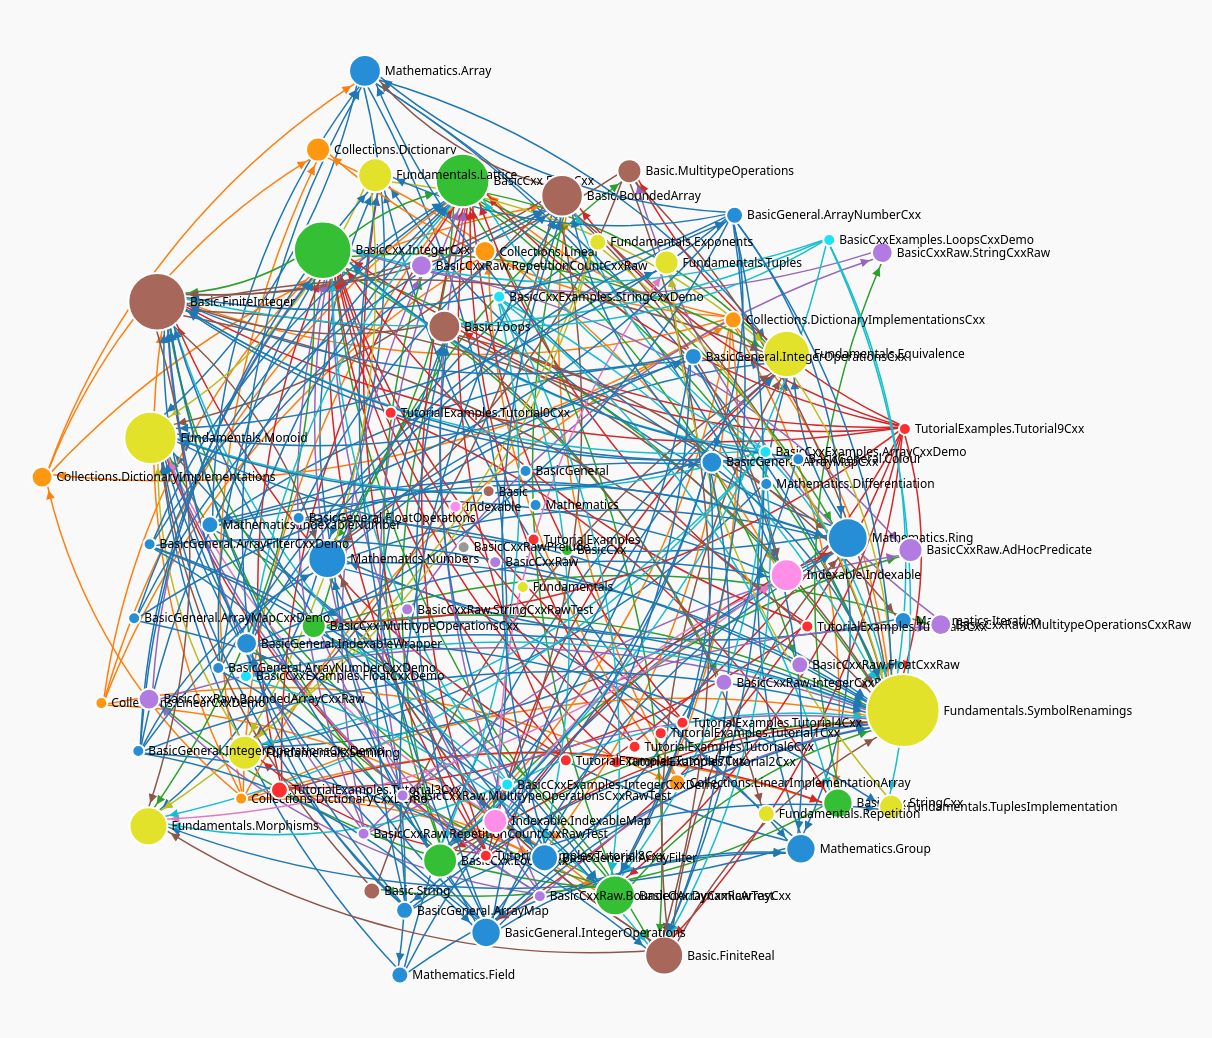
\includegraphics[width=0.75\textwidth]{magnolia-dependencies.png}
  \caption{
    Magnolia basic library dependencies visualized. Each colour represents a
    package, which contains several modules. The size of the nodes vary
    depending on the amount of dependents, (in degree), a module has.
  }
  \label{pic:magLib}
\end{figure}

Luckily, with \textit{D3}, we can mitigate some of the noise. In the picture
\ref{pic:depCont}, we can see the control-panel that our graph module has
created. With the control panel, we can zoom in and out on the graph,
(this can also be done with the mouse), reset our view. This is done with the
help of \textit{D3}, while the final button, find cycles, is implemented by
simply checking the input data for a cycle, and colouring it red with the help
of basic JavaScript and \gls{css}. The remaining sliders are specifically for
the graph ordering itself, where force strength, is with how much force nodes
exert on each other, and link distance is how far a link between two nodes
can/\textit{wants} to be. This, along with the node size scale, scaling how big
a node is depending on how many dependents it has, ensures this visualisation
tool can be used for other programming libraries, not just Magnolia.

\begin{figure}
  \centering
  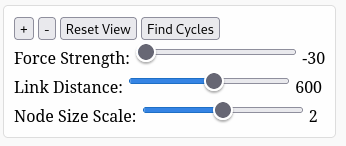
\includegraphics[width=0.45\textwidth]{dependency-viewer-controls.png}
  \caption{
    Control panel, with buttons and sliders for controlling the graph view
  }
  \label{pic:depCont}
\end{figure}

Furthermore, we can highlight the packages we care about, using the filter
panel the module created. In picture \ref{pic:depFil}, all the different
Magnolia packages have been detected, and their corresponding colour has been
added. We can then enable, or disable them.

\begin{figure}
  \centering
  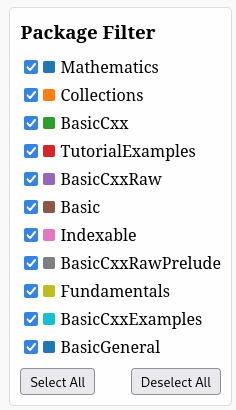
\includegraphics[width=0.45\textwidth]{dependency-viewer-filter.png}
  \caption{List of packages in the graph, that can be toggled}
  \label{pic:depFil}
\end{figure}

In the picture \ref{pic:depDis}, we can see the graph after we have disabled all
other packages, except the \textit{Fundamentals} package.

\begin{figure}
  \centering
  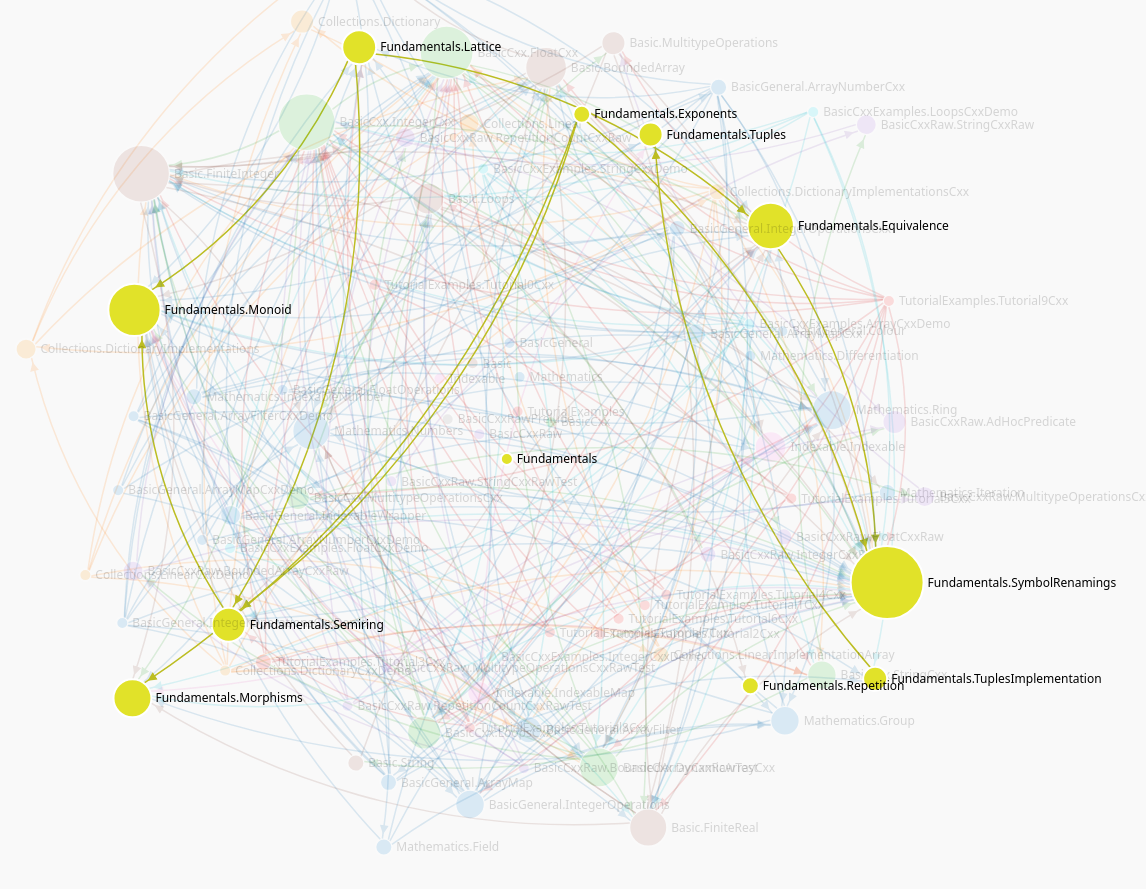
\includegraphics[width=0.75\textwidth]{magnolia-dependencies-filtered.png}
  \caption{
    Magnolia basic library, with just the \textit{Fundamentals} package
    highlighted.
  }
  \label{pic:depDis}
\end{figure}

\subsection{IDE Module Family}

\subsection{Caching}

There are two difficult problems in computer science\footnote{\url{https://martinfowler.com/bliki/TwoHardThings.html}}.
Cache invalidation, naming things and off-by-one errors. Compiler for
programming languages stores compiled code, such that it is not unnecessarily
re-compiled. Similarly, \gls{ide}s like \gls{intellij} or \gls{vscode} store the
application state between sessions, what files where opened, where in the files
one where, etc. In this \gls{ide}, something similar can be done, by using the
\textit{ide\_cache} module. This module declares a field on the state,
\textit{ide-cache}, which everytime the \gls{ide} exits, it writes to a file the
contents of the field, which it reads and adds to the state during the
\textit{PostInit}-event. That way, if existing modules are doing some state
change, they can be trivially refactored to use the cache field instead, by
simply pre-fixing all their paths with \textit{ide-cache}. In the dependency
visualizer, we can prefix the graph storing, with this, and then the generated
graph would be stored across sessions, ensuring a speedier visualisation
process, as we don't have to wait for an, relatively, expensive IO operation.

\subsection{IDE Framework}

An important aspect development, is separation of concerns. This is also
relevant for module development. A module that renders a \gls{dag}, should not
also be responsible for parsing a library and retrievieng the data to be
rendered. The same principle has been applied when developing prototype modules
for this \gls{ide}, the following modules are responsible for the \textit{view}
of the \gls{ide}:

\begin{enumerate}
  \item \textit{ide\_explorer}: Responsible for the file explorer
  \item \textit{ide\_framework}: Responsible for general layout
  \item \textit{ide\_pm}: Responsible for the menu bar
  \item \textit{ide\_tabs}: Responsible for the tabbing system
  \item \textit{ide\_errors}: Responsible in displaying module errors
\end{enumerate}

In the figure \ref{fig:ideLayout}, we have laid out the naming convention we
use when referring to different \textit{places} in the \gls{ide}.

\begin{figure}
  \centering
  \begin{tikzpicture}
  \node (window) [rectangle, draw, minimum height=7cm, minimum width=10cm] at (0, 0) {};
  \node (menu) [rectangle, draw, minimum height=0.5cm, minimum width=10cm] at (0, 3.25) {Menu};
  \node (tabs) [rectangle, draw, minimum height=0.25cm, minimum width=8cm] at (1, 2.75) {Tabs};
  \node (tab) [rectangle, draw, minimum height=0.25cm, minimum width=1cm] at (-2.5, 2.75) {Tab};
  \node (sidebar) [rectangle, draw, minimum height=6.5cm, minimum width=2cm] at (-4, -0.25) {Sidebar};
  \node (content) [rectangle, draw, minimum height=6.5cm, minimum width=8cm] at (1, -0.25) {Content};
\end{tikzpicture}
  \caption{\gls{ide} layout}
  \label{fig:ideLayout}
\end{figure}

The module \textit{ide\_pm}, being responsible for the menu bar at the top of
the \gls{ide}, has an \textit{easy} job, as it just simplifies the creation of
interactive \gls{ui} elements for other modules. With the dependency graph
visualization module, we can create a module which sends the initial Event that
triggers the graph visualization, and have the button be under the \textit{View}
dropdown content.

In picture \ref{pic:ideEx} we can see the ide\_explorer in action, showing the
Magnolia library visualized as a tree-like structure with collapsible folders.
These folders are rendered in the \textit{sidebar}, on the left. When we click
on the \textit{File}, a dropdown appears, where we can click on a button,
\textit{Open Folder}, which sends an Event to \gls{ide}\_fsa, the module in
charge of handling file system operations, where we get in \textit{response},
all the folders and files in the path we selected. Which we transform into
\gls{html}, and along with some \gls{css}, we get the collapsible folders.

\begin{figure}
  \centering
  
\includegraphics[width=0.25\textwidth]{ide-explorer.png}
  \caption{
    \gls{ide}-explorer module, showing the Magnolia library.
  }
  \label{pic:ideEx}
\end{figure}

There are also some icons, on files and folders, this is done using \gls{css},
in listing \ref{lst:ideEx}, we can see a snippet of this, since we are adding
the file exstension as a class attribute, we can very simply add
style-predicates to our files.

\begin{center}
  \lstinputlisting
    [ language=css
    , caption={
      Module for styling the file explorer, adding an latex icon to all files
      with the \textit{tex} exstension (\gls{css})
    }
    , label=lst:ideEx
    , firstline=152
    , lastline=154
    ]{./modules/ide\_explorer/ide\_explorer\_style.css}
\end{center}

\subsection{Editor Module Family}

The editor module family is coupled with the \gls{ide} framework, as using the
ide\_explorer module, we can open and edit files. By adding a \textit{click}
attribute to the files in the tree, we send an Event to \gls{ide}\_fsa, which
reads the file we clicked on. We know what file we clicked on, because each
\textit{click} attribute has sends an Event with their corresponding path. When
we get the texts contents of the file in response, we create an textarea with
the contents of the file added to it. In picture \ref{pic:editorModule} we can
see this in action, as the editor is created in the \textit{content} place, in
the center of the \gls{ide}, along with a \textit{tab}, with the name of the
file being edited as the title of the tab.

\begin{figure}
  \centering
  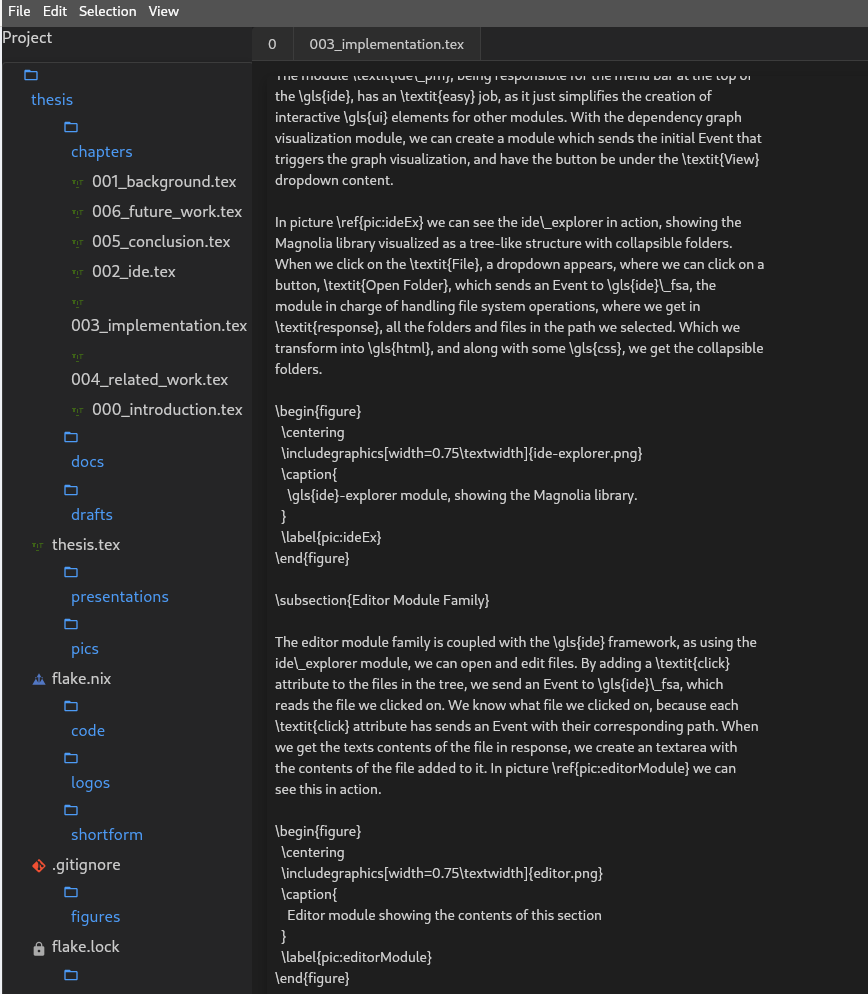
\includegraphics[width=0.5\textwidth]{editor.png}
  \caption{
    Editor module showing the contents of this section
  }
  \label{pic:editorModule}
\end{figure}

\subsection{Magnolia Language Server}

\todo{Implement a rudimentary Magnolia LS}


\chapter{Related Work} \label{cha:related}

\section{Existing module architectures in IDEs}

There exists module architectures in other \gls*{ide}s.


\subsection{Eclipse}

\gls*{ide}s are one of the most common application that supports extensions by
third-party code. \gls*{ide}s like Eclipse and IntelliJ are specialized for
working with Java, but they can still support other languages with the help of
modules. A module in Eclipse for instance, could extend Eclipse with
functionality like syntax highlighting, code completion, Go-to-definitions,
debugging, and more, for standard programming languages. A lot of this
functionality, comes from module-to-module extension, as in Eclipse modules can
extend modules, with the use of the \gls*{erpc}~\cite{eclipseRcp}.

\subsubsection{Eclipse Rich Client Platform}
\gls*{erpc} is a platform for building desktop applications. Eclipse being an
example of this platform in action. A plug-in could for example be responsible
for setting up the general \gls*{ui} layout, similar to our module,
\textit{ide\_framework}, and another plug-in could then modify this \gls*{ui} by
adding a file explorer, similar to our module \textit{ide\_explorer}.


\subsection{NetBeans}

An important part of NetBeans core architecture, is the NetBeans Module
\gls*{api}. This \gls{api} is responsible for supporting the
\textit{runtime environment}, which is the minimum amount of modules needed to
run the NetBeans application. A module in NetBeans is a JAR file, in which a
module can, amongst other things, list their public packages. This means that
other modules can directly invoke methods provided by this package.


\subsection{IntelliJ}

The extensibility IntelliJ has, is achieved by its extensions points
architecture. This is an \gls*{api} for plugins to integrate with the
\gls*{ide}. Plugins use this \gls*{api} to register their implementations, which
the \gls*{ide} then use. Between different versions of IntelliJ, plugins may be
broken, due to a breaking change in their plugin \gls*{api}.


\subsection{Visual Studio}

There are two kinds of extensions in Visual Studio, \textit{VSPackage} and
\textit{MEF} extensions. \textit{VSPackage} are mainly used to extend
functionality like tool windows and projects, while \textit{MEF} extensions are
used to customize the text-editor.

\subsection{Visual Studio Code (VS Code)}

Visual Studio Code is an extensible \gls*{ide}. It achieves this extensibility
with its extension \gls*{api}. This \gls*{api} allows for extensions to modify
the look and behavior of the \gls*{ide}. In fact, many of the core \gls*{ide}
features are possible due to built-in extensions.

\subsection{Emacs}

Emacs\footnote{\url{https://www.gnu.org/software/emacs/}} is an extensible text
editor. Almost all of Emacs functionality is achieved by writing code in Emacs
Lisp, a dialect of Lisp\footnote{\url{https://lisp-lang.org/}}. Unlike other
\gls*{ide}s, Emacs does not restrict modules to a certain \gls*{api}, instead
they are free to modify anything, as the functionality from the Emacs Lisp,
\textit{sits} atop of a core written in C, which abstracts away platform
specific code, and enables Emacs to be turned from an a \textit{simple} text
editor, to write and send emails, multimedia management and much more. Another
interesting thing about Emacs, is that all files are in \textit{buffers},
meaning the representation of a file shown to the user, is not necessarily the
contents of the file, some rendering is can be done by a plugin, before the file
contents is shown to the user.


\subsection{Theia}

\say{The Theia \gls*{ide} is a modern \gls*{ide} for cloud and desktop built on the Theia Platform}\footnote{\url{https://theia-ide.org/}}.

Eclipse Theia is a highly extensible \gls*{ide}, supporting \textit{extensions}
from VS Code, their own extensions and plugins, and \textit{headless} plugins.
Theia differentiates between extensions and plugins, where a plugin is installed
during runtime, and an extension is installed during compile-time.

Theia reuses components from VS Code, like their extensions \gls*{api}, which
enables them to support VS Code extensions. Theia plugins share similarities
with VS Code extensions, but are not restricted to \textit{just} the VS Code
\gls*{api}.

Theia's extensions are designed to add or remove existing core functionality in
Theia. They also have access to the entire core \gls*{api}.

An headless plugin runs without access to the frontend, meaning they are suited
for \gls*{cli} interactions, or similar use cases where a frontend is not
needed.

Theia is both a desktop \gls*{ide} and a web \gls*{ide}. Where there is no real
distinction between the two, both abstracting it to a frontend and backend. This
is similar to our zero-core \gls*{ide}, as we can make this abstraction due to
our usage of a web view for the desktop \gls*{ide}.


\section{Graphical User Interface development} \label{sec:guid}

A common complexity within application development, is \gls*{gui} development.
Using the \gls*{mvc}-pattern as an example, \gls*{gui}s can represent structures
such as lists, which users might want to manipulate in some fashion, like
appending or rearranging the items in the list. Managing such a change,
especially one that involves \gls*{gui} widgets can be a challenge, since a
change in the view should be reflected in the model, and encoding this can be
very involved.

Another issue in \gls*{gui}s is optimizing performance in regard to events
triggered by user actions, such as scrolling, resizing or typing. These events
could happen many times in a second, while in theory user speed is trivial for a
computer to keep up with, there are instances where a module family could be
quite large, meaning many different modules are triggered by the same event many
times. There are techniques, called event coalescing, for handling this, like
debouncing and throttling.

\paragraph{Debouncing} Debouncing is a technique where you delay the sending of
an event until after some time period $T$ has passed. Once the event is triggered
$T_0$ starts counting down. If the same event is re-triggered while $T_0 > 0$,
$T_0$ is reset by $T_0 = T$. If $T_0 = 0$, then the event is sent. Ensuring that
$T$ is not too large, is important, as if $T$ is above some threshold, the user
of the \gls*{gui} will notice, and it will make the application \textit{feel}
slow.

\paragraph{Throttling} Throttling is a similar technique to debouncing, except
instead of delaying the event by some time $T$, the event is only sent when
$T_0 = 0$. Meaning the event is sent at regular intervals, and could be sent at
the exact same point in time when the user triggered the event, or it could
happen at most, $T$ units after the user action.


\subsection{Flushable promises}

Debouncing and throttling work in less complex \gls*{gui} structures, but as the
amount of features in an application increases, the complexity will also
increase. These event-coalescing-strategies are a source of subtle bugs, as
event coalescing can easily break modularity. In a \gls*{jsms}, this issue could
be solved by using \textit{flushable promises}~\cite{flush}. This could have
solved our issue, where we had some event handler that took noticeably longer
time to return, but since this was a Rust module, we could \textit{solve} this
by doing this computation on another thread. If it was a JavaScript module we
could have solved it by using \textit{flushable promises}.

If we implement a \gls*{ls}-client in JavaScript, \textit{flushable promises}
could allow for a smoother experience, as things like \textit{looking up}
renaming in a Magnolia project is a more involved process for the compiler,
and in larger projects, could take a noticeably long time.


\subsection{Multi-way Dataflow Constraint System}

Luckily, there exists frameworks that make this task easier.
\textit{WarmDrink},~\cite{warmDrink, dslMdcs} is a JavaScript framework that
allow a developer to declarative specify structural changes in an application.
The framework can guarantee \gls*{gui} behavior, by utilizing a \gls*{mdcs},
ensuring it can create constraint systems. A constraint system is a
representation of how different variables are dependent on eachother. If one
variable is needed in the computation of another, they have a dependency
relation. By using a \gls*{dsl}, a developer can declare a constraint system.
But, similar to how working on our \textbf{Instruction}-set without tooling is
quite complex, tools have been created to ease the creation of such constraint
systems~\cite{toolMcds}. Given how WarmDrink is a JavaScript framework, it is
quite well suited for the web, aswell as our \gls*{ide}. A runtime system
specifically for a \gls*{mdcs} could be implemented for JavaScript modules.
Furthermore, there also exists a Rust implementation of this framework, which
means a similar system can be created for Rust modules.

\section{Automated testing}

Due to the extensive modularity of the application, all modules can be tested
individually, by \textit{mocking} the expected state and events. This means that
breaking changes in one module can be detected before \gls*{e2e} testing, which
is expensive. But this can only verify the general logic of a module and module
family, not the UI. To achieve such automation, one could rely on an automated
testing framework, like the one in~\cite{autoUi}. Or if one is working with a
\textit{simple} JavaScript runtime, one could use third party software like
\textit{Playwright} for creating tests, as it can auto generate the \gls*{dsl},
while the developer uses the module or entire \gls*{ide} if it is an \gls*{e2e}
test. This would help a module developer to discover behavior that a user might
not expect~\cite{leastGui}.


\section{Syntactic Theory Functor}

\gls*{stf} is a framework for creating, reusing and restructuring
specifications\cite{stf:haveraaen:2020}, specifications from algebraic
specification languages like CafeOBJ~\cite{cafeObj}. \gls*{stf}s are also used
by the new Magnolia compiler\footnote{As of May 2025, still in development}, to
resolve renaming in Magnolia and \textit{flattening} of the \gls*{asr} to be
shown to the developer \cite{wiig}.


\section{Abstract algebra}

Magnolia is a kind of algebraic specification language, like CafeOBJ~\cite{cafeObj}.
An algebraic specification language, is a language where one can develop
similarly as to how one might create an algebraic structure. We specify some set
and some functions that take elements from the set as inputs. Finally, we
specify the behavior of our functions, if they are associative, if there are any
predicates that the arguments to the functions need to fulfill, etc. As shown in
the development of this \gls*{ide}, this can be quite useful way of thinking.


\section{Language workbenches}

Language workbenches are tools for creation and use of computer languages~\cite{lwb}.
An \gls*{ide} is a kind of language workbench, as it can be used both for a
language, as described in this thesis, but also for creating languages, as this
too is a software project. More specific are the tools created by JetBrains,
Meta-Programming System (MPS)\footnote{\url{https://www.jetbrains.com/mps/}},
for creating programming languages, specifically \gls*{dsl}s. What makes tools
like MPS different from standard \gls*{ide}s, is that in standard \gls*{ide}s we
work on the source file of a program, while language workbenches work on the
\gls*{ast} of the program. Programming languages were made so that we
programmers could read closer to how we think, than how a computer thinks. So
before a computer can run our code, it needs to be translated. Generally, this
translation is done by parsing the source file into some tree-structure, and
then interpreting that tree, transforming it into an \gls*{ast}.

So language workbenches then, enables a developer to work on this abstract
representation of the language one is creating.


\section{Language Server}

The most important features in a modern \gls*{ide} are possible due to the
\gls*{lsp}\footnote{\url{https://microsoft.github.io/language-server-protocol/specifications/lsp/3.17/specification/}}.
\gls*{lsp} is a protocol for a language server and editor, (the client), in
which they communicate, allowing for many of the features mentioned in section
\ref{sec:ide}, and explicitly mentioned in table \ref{tbl:ide}. \gls*{lsp} being
the standard since the 2020s, is a sign of modularity being preferred, as now a
single \gls*{lsp} can be created, and used across several different
applications, like IntelliJ, VS Code and \gls*{vim}. While useful for
\textit{standard} language, this is the limiting factor when it comes to
supporting experimental languages, as not only does a new set of protocols need
to be appended to a language server, the editor itself needs to be changed to
actually use these protocols. This creates a lot of work, for both the
\gls*{ide} developer and for the compiler developer. Here is where a modular
approach can help both. If some new functionality or feature is added to the
experimental language, this off course means the compiler/interpreter has to be
expanded and/or modified, but for the \gls*{ide}, a module could be added and/or
modified to utilize this change, instead of having to change the entire
application.

\begin{table}[]
  \centering
  \caption{\gls*{ide} features enabled by \gls*{lsp}}
  \label{tbl:ide}
  \begin{tabular}{|l|l|}
    \hline
    IDE Feature & \gls*{lsp}-method \\ \hline
    Go to Declaration & textDocument/definition \\ \hline
    Go to Implementation & textDocument/implementation \\ \hline
    Auto-completion & textDocument/completion \\ \hline
    Hover & textDocument/hover \\ \hline
    Warnings & textDocument/publishDiagnostics \\ \hline
    Rename & textDocument/rename \\ \hline
  \end{tabular}
\end{table}

An example of this in action, say a developer is working on a file
\textit{main.ts}, in their Typescript project. They hover over a type imported
from, and defined in \textit{types.ts}. This is what happens:

\begin{enumerate}
  \item The editor detects the user is hovering over a \textit{special} word
  \item The editor sends a request to the Typescript \gls*{ls}
  \item The \gls*{ls} responds
  \item The editor formats the response into a small window showcasing the
    documentation and implementation of the type
\end{enumerate}


\chapter{Conclusion \& Discussion} \label{cha:conclusion}

We will discuss some of the issues encountered when developing this modular
\gls*{ide}, and make a conclusion from our hypothesis \ref{hyp:modular}.


\section{Modular development} \label{sec:mod-dev}

In this thesis, we have shown that developing against a zero-core modular
architecture is trivial. By utilizing separation of concerns, a module developer
needs to only understand the feature they want to extend, or if it is an
entirely new feature, find out what has been done before.


\subsection{Unstable API}

Developing against an unstable \gls*{api} is difficult, when developing a module
architecture, it is like an unstable \gls*{api} when it is not \textit{mature},
e.g. when it does not have settled modules to develop against. Since this is
the case, there are a lot of issues with the existing modules, making the user
experience less than competing \gls*{ide}s. Most of these are minors, and can be
fixed with some minor revisions to the existing modules, for instance, when
closing the \gls*{ide}, unsaved changes are discarded, with no information given
to the user. Or how what project a user was working on, is not saved between
instances, so a user has to re-open the project they worked on. This is a side
effect of the development plan, and not the architecture. To fully test out this
architecture, it was thought that a wide range of modules should be implemented,
to quickly iron out issues with the implementation of the architecture, and to
figure out what functionality Tauri has, that we can expose, like the file
selection.

So not only were modules needed to cover the necessities to qualify as an
\gls*{ide}, but they were also needed to \textit{test} the implementation. Not
having a developer dedicated to only implement modules, meant that module
development was usually dropped for other things. As every time a module where
worked on, it would eventually lead to a discovery, that the current \gls*{api}
needed some change, which would enable the module feature to be easier
implemented. A concrete example of this, is the editor module.
An essential part of an editor, in an \gls*{ide} at least, is being able to
utilize a \gls*{lsp}. Most of the communication between a client and \gls*{ls},
require information about \textit{where} the user is in the text. This
information is available in a \textit{textarea}-element, but some change to how
Events are sent were needed. In standard JavaScript development,
\textit{eventListeners} can be specific to the \gls*{html}-element they are
applied to. The same is not possible in our \gls*{api}, as Events are generic.


\subsection{Module deprecation}

Instead, we made Events gather information about the \gls*{dom}-Event they were
triggered by, so in the case of \textit{click} attribute, we know the
\gls*{dom}-event is of type \textit{MouseEvent}, which can give us some,
information. And if the \textit{target}, (a field on \textit{MouseEvent}) is an
instance of \textit{HtmlInputElement} or \textit{textarea}, we know that the
\textit{selectionStart} and \textit{value} field exist on the target. With
which, we can manually calculate the position of the click. Implementing this
meant adding a breaking change to the \gls*{api}, which deprecated different
modules, so more time was spent on re-implementing them.


\section{Lacking language agnosticism} \label{sec:lla}

Not really achieved, because we cannot syntactically translate between a
JavaScript Module and a Rust Module. This is due to the differences between the
utility libraries created for \gls*{jsms} and \gls*{rsms}. When \gls*{jsms} modules
where created, they were primarily made for using existing JavaScript libraries,
to showcase this interoperability. So, much of the \gls*{html} elements were
created using JavaScript, so the utility library primarily focused on this,
having builder pattern for creating \gls*{html}. There is a similar builder
pattern in the Rust utility library, but it is not a one-to-one mapping, meaning
there are some semantic differences between two modules doing the same.

But \textit{installation} of the modules also differ. In JavaScript, module
developers can simply invoke the \textit{installModule} function, with their
created module, to install the module. The reason this works, is that when we
bundle all JavaScript modules during compile time, it ends up as a script-tag in
the \gls*{dom}. The same is for the case of runtime JavaScript modules. The
result, in either case, is that the entire contents of the JavaScript file is
evaluated, meaning even though we are simply importing a JavaScript file, and
not explicitly invoking anything, it ends up with the modules being installed.

This is not the case in Rust, importing another Rust crate does not mean we
invoke it. That is why we need the extra steps of creating a
\textit{ModuleBuilder}, which has to implement the \textit{ModuleBuilder} trait,
so that we can build the module.


\section{Foreign modules} \label{sec:fm}

Languages like Gleam and PureScript, which compile directly to JavaScript can
be trivially added. But for languages that can target the C-\gls*{abi}, this is
less trivial. This is because of how the core-\gls*{ide} was designed. We decided
to use a \textit{Rust-y} approach, meaning we utilized many of the features that
made interoperability between the Rust-\gls*{abi} and C-\gls*{abi} more complex.
An example of this, can be found in the listing \ref{lst:value} and
\ref{lst:rsValue}, where we have the \textit{standard} value variant, and then
the \textit{C-safe} variant.

\begin{code}[H]
  \lstinputlisting
    [ language=Rust
    , caption={Value variant (Rust)}
    , label=lst:value
    , firstline=19
    , lastline=31
    ]{./libs/rust/core-std-lib/src/state/mod.rs}
\end{code}

\begin{code}[H]
  \lstinputlisting
    [ language=Rust
    , caption={C-safe value variant (Rust)}
    , label=lst:rsValue
    , firstline=16
    , lastline=21
    ]{./libs/rust/foreign-std-lib/src/state/rs\_state.rs}
\end{code}

Note the \textbf{\#[repr(C)]} macro attribute, and the two fields,
\textit{kind} and \textit{val}. The macro attribute specifies to the Rust
compiler that it should \textit{do what C does}. This is in regard to order,
size and alignment of fields of a structure. Since we cannot have the same enum
structure as we can in Rust, the work-around was an enum that specifies what
kind of value we are working with (\textit{val}), and a union, that holds the
specific value. A union in both C and Rust, has the same size in memory, as the
largest possible value it can store. In listing \ref{lst:rsValueUnion} we can
see this union. Accessing a field is inherently an \textit{unsafe} action, as we
cannot tell the compiler if the bytes we are reading are actually and integer,
or is a list of values. We can see this, as in the listing
\ref{lst:rsValueUnsafe}, on line three, we have to use the \textit{unsafe}
keyword in Rust, which essentially means the compiler cannot promise what we are
doing in this code block is \textit{valid}.

\begin{code}
  \lstinputlisting
    [ language=Rust
    , caption={Union used to hold the values the C-safe value can have (Rust)}
    , label=lst:rsValueUnion
    , firstline=134
    , lastline=144
    ]{./libs/rust/foreign-std-lib/src/state/rs\_state.rs}
\end{code}

\begin{code}
  \lstinputlisting
    [ language=Rust
    , caption={
      Accessing a value in the C-safe value variant is inherently unsafe (Rust)
    }
    , label=lst:rsValueUnsafe
    , firstline=53
    , lastline=59
    , numbers=left
    , numberstyle=\tiny\color{gray}
    ]{./libs/rust/foreign-std-lib/src/state/rs\_state.rs}
\end{code}

But with the starting point of the runtime Rust module system, a C module system
could be developed. One would just have to ensure that the differences between
the modules are syntactical, and not semantics.


\section{Ad-hoc solutions for lackluster API} \label{sec:lackluster}

As mentioned, there is an issue in the current \gls*{api} on maintaining
consistency between the \gls*{ui} in the frontend, and the \gls*{ui}
representation the \gls*{rsms} has access to. This means that there is no
good way to achieve saving of an edited file. But this is still a feature the
editor module supports. The way saving was implemented, was to add plain
JavaScript to the save button, where when the user presses it, the contents
of the textarea are sent to the \gls*{ide}\_fsa module, which can save the
contents. This is an action that bypasses the core \gls*{ide}, which was
necessary due to the lacking \gls*{api}.


\section{Conclusion} \label{sec:conclusion}

Developing against an unstable \gls*{api}, means that modules can be
deprecated. It also means that module language agnosticism can quickly
disappear, since that depends on having multiple different libraries in sync
with an unstable one. In fact, many of the issues that we have claimed to be
innate with \gls*{ide}s, appear in this stage of our modular architecture. But,
our \gls*{api} is bounded, we have some types, and some operation on those
types. We have chosen to have a larger set of operations, simply due to the
fact that this enhances the module developer experience. But to figure out what
utility functions are necessary, we need to develop modules. Once the
satisfactory functions are developed, our \gls*{api} is stable. Which means
modules are no longer in danger to be deprecated. Which means that module
language agnosticism can be corrected for. Finally, this means that future
changes coming from the outside, being a paradigm shift on what is necessary to
have in an \gls*{ide}, or a language, the necessary modules can quickly be
developed and integrated into the current solution.



\chapter{Future Work} \label{cha:future}

Would've, could've, should've.


\section{Technical debt}

It just piles and piles and piles on.

\begin{enumerate}
  \item Missing tests
  \item Not a total mapping between \gls*{dom} stuff and the Rust counterpart
  \item Inconsistent \gls*{ui}
\end{enumerate}


\subsection{Testing}

No unit tests for the TypeScript side, no integration testing between the
frontend and backend.

There should be tests made to ensure that a module behaves the same, if written
in Rust or JavaScript. This can be an issue, because the way a module interacts
with the \gls*{ide} is through a core, which is implemented separately for the
different module systems. Test modules should be made, ensuring that the end
state of the \gls*{ide} is the same, when the module does the same action. But
this would require the modules being semantically the same for the different
test cases. In any case, difficult to ensure all edge cases have been covered.

\subsection{Language agnosticism}

Steps should be made to mitigate the shortfall of this solution, with regard to
language agnosticism. The differences in installation for \gls*{rsms} and
\gls*{jsms} are mainly due to how trivial it is to install JavaScript modules,
compared to Rust modules. \gls*{jsms} should enforce a similar system of module
building as \gls*{rsms}, not only to ensure less semantic differences, but also
to ensure safety, as restricting the \gls*{jsms} is good.

\subsection{Attribute and instructions}

Can't remove or change eventListeners currently. This is because to remove an
EventListener, the exact same function passed to the \textit{addEventListener}
must be used, which means a reference to this function needs to be stored, but
having two or more of the same type? It can get confusing for a module developer
of what should actually happen.

\subsection{Keypresses}

A common feature of \gls*{ide}s is being able to have certain keybindings for
different actions. For example, in \gls*{vscode}, one can hit \textit{CTRL}
$+$ \textit{n} to open up a new tab, with a new file. This system is not yet
possible in the \gls*{ide}, but this is due to a lack of a supporting module
family. But, given that this is a common feature in \gls*{ide}s, this should be
a priority.

\subsection{Inconsistent UI}

Difficult to keep the \gls*{ui} representation consistent with the \gls*{dom}.
An example of this, is that the \gls*{ui} representation in the \gls*{ide} does
not store information like the possible \textit{value} an \gls{html} might
have. So for the editor module, there is no efficient way to know what text is
in the editor. Another example, is for the module installer, there is no way for
the module to \textit{query} the \gls*{ui} for information about the form it
presents the user, seeing what values are in the fields. A workaround to this
was used, where depending on what element an \textit{eventListener} was added
to, the sent event would be \textit{sticky}, meaning it would add extra
arguments to the \textit{args} field of the Event, like attribute information,
id, value, etc. But this would not update the \gls*{ui} stored in the
\gls*{ide}, but rather give modules a peek at the current \gls*{ui} state. A
better solution would be to somehow keep track of \textit{all} user interactions
to the \gls*{dom}, and somehow bubble these changes down to the backend, where
the \gls*{ui} representation is managed.

\subsection{Unify the tooling}

A \gls{cli} tool should be made for users to add compile-time modules.
Currently, a user has to specify what kind of module they are adding, the
language and package manager if it is a JavaScript module. This is trivial to
detect by a program. A user should be able to simply invoke the tool with
either a URL or a path to the module, and then the tool can infer what kind of
module it is, and add it to the configuration file correctly. The same tool
should also include the other tooling, like generating the module dependency
graph.

\section{Modular editor}

The prototype editor module develop for this \gls*{ide} is subpar compared to
existing ones. A new one should be developed, in tandem with a \gls*{ls} client.
This will ensure that this \gls*{ide} can support more languages. This editor
should then utilize existing technology that is already used by other
\gls*{ide}s, like the tree-sitter\footnote{\url{https://github.com/tree-sitter/tree-sitter}}
parsing system, which amongst other things, can help with syntax highlighting.


%%=========================================

% Alternative 1 of printing glossaries & acronyms
%\renewcommand{\glossarypreamble}{\footnotesize}
%\printglossary[style=super, type=\glsdefaulttype] \let\cleardoublepage\clearpage
%\printglossary[style=super, type=\acronymtype]


%Alternative 2
%Simplified way of printing glossaries, slower than alt 1, but has better compatibility
\printnoidxglossaries

% Include more appendices as required.
%%=========================================
\clearpage
\DeclareRobustCommand{\VAN}[3]{#3}
\addcontentsline{toc}{chapter}{Bibliography}

\printbibliography

\appendix
\titleformat{\chapter}[display]
  {\normalfont\large\bfseries}% <- font for label "Appendix A", default \huge
  {\chaptertitlename\ \thechapter}
  {20pt}
  {\large}% <- font for title, default \Huge

\chapter{Optimizing instructions sets} \label{app:a}

The following appendix discusses how we can optimize an instruction set. When we
use the term \textit{optimize}, we mean to reduce the amount of instructions.
This can be achieved in a few different steps. \textbf{Instruction} is a
recursive data type, parameterized by \textbf{T}. Since an \textbf{Instruction}
form a monoid\footnote{See section \ref{sec:moD3} in chapter \ref{cha:impl}}
structure, we know for any \textbf{Instruction} variant, there exist an inverse,
giving us the unit. The goal of this optimization, is to see if an
\textbf{Instruction} tree contains any inverses.

\begin{enumerate}
  \item Flatten the Instruction
  \item Register how many times a field is modified
    \begin{enumerate}
      \item Turn unnecessary Instructions into NoOps
    \end{enumerate}
  \item Filter out NoOps
  \item Unflatten the Instructions
\end{enumerate}

An \textit{unnecessary} operation is one that leads to an \textbf{NoOp}, which
is the case of inversable \textbf{Instruction}s. The optimalization function
is not parameterized by a strict variant of \textbf{T}. In the \gls*{ide} the
\textbf{Instruction}s are parameterized by \textbf{Value}, \textbf{Html},
\textbf{Attr} and \textbf{String}. The last three are specific to \gls*{ui}
modification, and the last two are modifications on specific \textbf{Html}
instances. This means that if an \textbf{Instruction} parameterized by
\textbf{Html}, is of the \textbf{Rem} variant, we know all other \gls*{ui}
\textbf{Instruction}s pertaining to the removed \textbf{Html} variant are
\textbf{NoOp}s.

\begin{code}[H]
  \lstinputlisting
   [ language=Rust
   , caption={Instruction (Rust)}
   , label=lst:aInst
   , firstline=4
   , lastline=16
   ]{./libs/rust/core-std-lib/src/instruction/inst.rs}
\end{code}

In Rust we can have generic data types, as shown in listing \ref{lst:aInst}, by
the type parameter, $T$, but we have to restrict the type $T$ to a type that
implements the trait \textbf{PartialEq}, which means we can use equality on it.
We need this restrictions, because the attribute macro \textbf{Instruction} has.
These macros generate the needed code to implement the different traits:

\begin{itemize}
  \item Debug: Enables the implementer to be printed to \textit{stdout}
  \item Default: Implements a default variant of the implementer type, in this
    case, NoOp
  \item Clone: Implements a simple \textbf{clone} method, to create an owned
    instance of a borrowed value
  \item Deserialize \& Serialize: Implements the needed methods for encoding
    and decoding a variant to a \gls{json} representation
  \item TS: Enables automatic TypeScript type generation of the variant
\end{itemize}

We first start the optimalization step, by removing all NoOps, and then
flattening the instructions, by using the \textbf{opt} and \textbf{flatten}
methods, shown in listings \ref{lst:opt} and \ref{lst:flatten} respectively.

\begin{code}[H]
  \lstinputlisting
   [ language=Rust
   , caption={
     Opt method (Rust): Uses a match statement and a guard to match on a
     \textit{slice}, (reference to a Vec). The guard lets us add a predicate to
     our branch, in this case, if y \textit{matches} an NoOp. If it is an empty
     slice, it's a NoOp, otherwise, it will be an Instruction with all NoOps
     recursively removed.
   }
   , label=lst:opt
   , firstline=119
   , lastline=151
   ]{./libs/rust/core-std-lib/src/instruction/opt.rs}
\end{code}

\begin{code}[H]
  \lstinputlisting
   [ language=Rust
   , caption={
     Flatten method (Rust): Note the lack of return statements, this is because
     the last expression in a function in Rust, is returned, if the expression
     does not end with a semicolon.
   }
   , label=lst:flatten
   , firstline=17
   , lastline=26
   ]{./libs/rust/core-std-lib/src/instruction/opt.rs}
\end{code}

In listing \ref{lst:count}, we then iterate over each instruction in the
sequence, and mapping each field and value to a counter. If it's an Add
instruction, the counter is incremented, if it's a Rem instruction, the counter
is decremented. We don't have a way to inform the compiler that we have removed
all NoOp and Then instructions, and we need complete match-statements, so we add
a catch-all with an \textit{unreachable} macro, which will \textit{panic} with
the supplied message. This is commonly used to represent a state that is
unreachable, but something the compiler can't prove.

\begin{code}[H]
  \lstinputlisting
   [ language=Rust
   , caption={Modification counting (Rust)}
   , label=lst:count
   , firstline=50
   , lastline=79
   ]{./libs/rust/core-std-lib/src/instruction/opt.rs}
\end{code}

Finally, in the listing \ref{lst:fold}, we \textit{unflatten} the sequence of
instructions, and check the count for each Add and Rem Instruction. If it is
above $0$, then that means we have added that field-value pair more times than
removing it, but we can still only add it once, so we set the count to $0$, and
return a Then instruction, since we have the accumulated instructions along with
the current Add instruction. If the count is less than $0$, then it means we are
removing it more times than adding it, similarly, we can only remove it once, so
we set the count to $0$, and combine the accumulated instruction, with the Rem
instruction. Because of our \textbf{combine} implementation, we can be sure that
the initial NoOp element is removed as soon as possible.

\begin{code}[H]
  \lstinputlisting
   [ language=Rust
   , caption={Instruction folding (Rust)}
   , label=lst:fold
   , firstline=81
   , lastline=112
   ]{./libs/rust/core-std-lib/src/instruction/opt.rs}
\end{code}

\end{document}
